%------------------------------------------------------------
% thesis completion seminar - Andy Taylor 
%------------------------------------------------------------
\documentclass{beamer}
\usepackage[utf8]{inputenc}
\usepackage{style/uom_beamer}
\usepackage{multicol}

%\newcommand{\figureInit}{\begin{figure}[h]\centering}
%------------------------------------------------------------------------ 
% shortcut text
%------------------------------------------------------------------------ 
\newcommand{\TITLE}{`TITLE'}
\newcommand{\ALTTITLE}{`ALT TITLE'}
\newcommand{\BOM}{Australian Bureau of Meteorology}
\newcommand{\LTE}{\textbf{\texttt{LTE}}}
\newcommand{\ATGF}{\textbf{\texttt{ATGF}}}
\newcommand{\ATGP}{\textbf{\texttt{ATGP}}}
\newcommand{\SSH}{\textbf{\texttt{ssh}}}
\newcommand{\BL}{\textbf{\texttt{Bluelink-OceanMAPS}}}
\newcommand{\MOM}{\textbf{\texttt{MOM}}}
\newcommand{\ROMS}{\textbf{\texttt{ROMS}}}
\newcommand{\GODAE}{\textbf{\texttt{GODAE}}}
\newcommand{\OGCM}{\textbf{\texttt{{OGCM}}}}       %{\textbf{\texttt{OGCM}}}
\newcommand{\OFAM}{\textbf{\texttt{{OFAM}}}}
\newcommand{\OFAMHR}{\textbf{\texttt{{OFAMHR}}}}
\newcommand{\NWP}{\textbf{\texttt{NWP}}}
\newcommand{\OTIS}{\textbf{\texttt{OTIS}}}
\newcommand{\GOOS}{\textbf{\texttt{GOOS}}}
\newcommand{\obc}{\textbf{\texttt{obc}}}
\newcommand{\ANTT}{\textbf{\texttt{ANTT}}}
\newcommand{\CTE}{\textbf{\texttt{CTE}}}
\newcommand{\SAL}{\textbf{\texttt{SAL}}}
\newcommand{\AG}{\textbf{\texttt{ACCESS-G}}}
\newcommand{\AR}{\textbf{\texttt{ACCESS-R}}}
\newcommand{\ER}{\textbf{\texttt{eReefs}}}

% add DRAFT water mark
\usepackage{draftwatermark}
\SetWatermarkText{DRAFT} 
\SetWatermarkLightness{0.98}
\SetWatermarkAngle{45}
\SetWatermarkScale{1.2}
                % draft watermark
\begin{document}
%------------------------------------------------------------
% metadata  ..note syntax: [short]{long}
\title[Tides and sea level forecasting]{Sea level forecasts, tide prediction and mesoscale operational oceanography in Australia}
%\author[Andy Taylor]{Andy Taylor} 
\newcommand{\department}{School of Earth Sciences}
\newcommand{\university}{\textsc{The University of Melbourne}}
\newcommand{\BoM}{\sc Australian Bureau of Meteorology}
\institute[]{\university \par \department  \par and \par \BoM}
\date[Completion 2021]{Completion Seminar 21-03-2021}
%------------------------------------------------------------
% title slide 
\frame{\titlepage}
%------------------------------------------------------------
% auto overview for every section in style file
%------------------------------------------------------------
% sections 
\section{Summary}
\begin{frame}
\frametitle{Abstract}

Part-time thesis with publication:
\begin{itemize}
    \item conceptual intersection of tides and mesoscale oceanography
    \item motivation towards \bold{seamless} forecasting
    \item background of simulation system upgrades
    \item new methods for combining, evaluating and delivering nominally ``tidal'' sea level information
    \item focus on representation and incompatibility
     updates 
\end{itemize}

\end{frame}
%--------
\section{Intro}
\begin{frame}
\frametitle{Brief intro yarn}
Super brief personal story.

Why this topic?

% ;prelude 1:  the perspnal yarn
% renewables,  fluids - HPS
% travel 
% sailing pelican -> antt!
% naval engineering -> renewables
% BoM encounters
% ...wind obs for bankable truth
% ...ocean forecasts -> but 'nontidal'!?
% Academic
% ...wave interest via offshore -> AlexB
% ...reality $$ job or scholarship
% Bluelink
% ...inherit sea level report
% ...expand 

\end{frame}
%-----------------------------------------
\begin{frame}
\frametitle{Scope - exciting and mundane sea level}
\begin{itemize}
    \item Desktop study
    \item Operational system and data wrangling
\end{itemize}
\end{frame}
%-----------------------------------------
\begin{frame}
\frametitle{Scales}
\begin{minipage}{0.45\textwidth}
    \begin{figure}      
    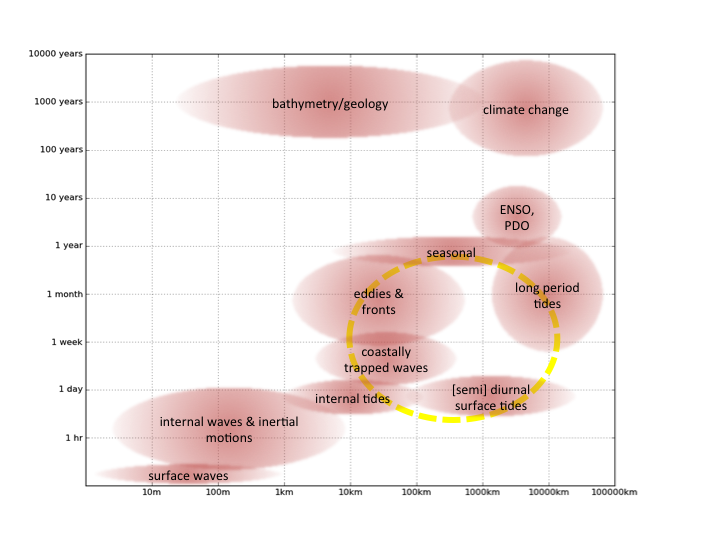
\includegraphics[width=\textwidth]{figures/diagrams/ocean_scales.png}
    \end{figure}
\end{minipage}
\hfill
\begin{minipage}{0.45\textwidth}
    \begin{figure}      
     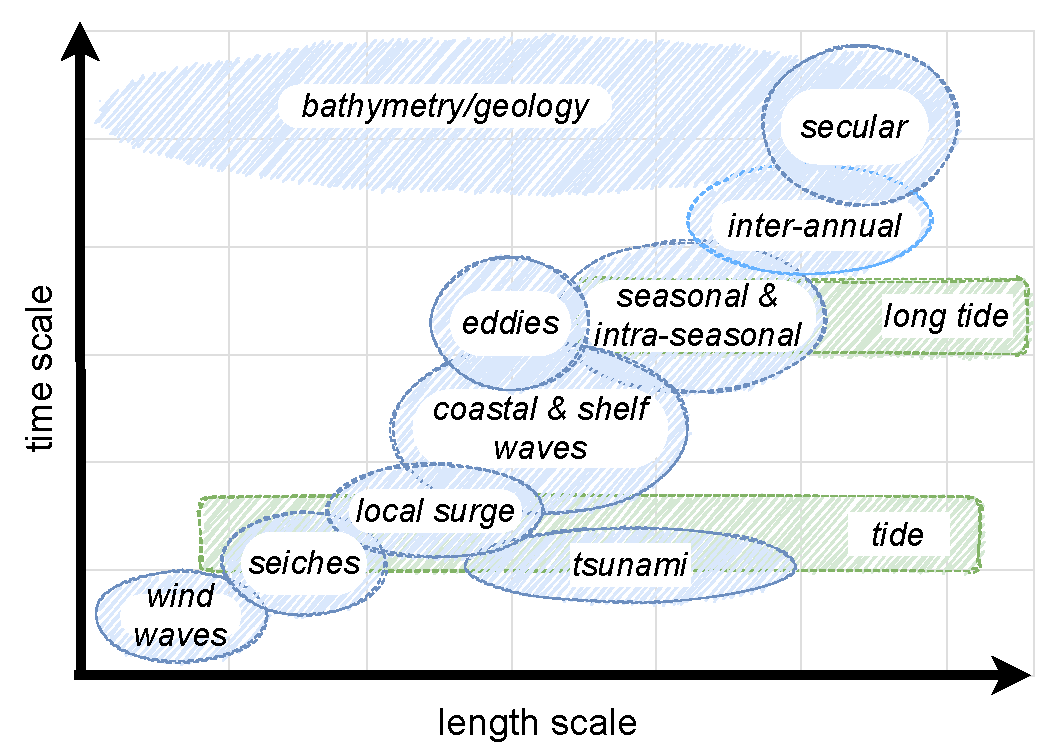
\includegraphics[width=\textwidth]{figures/diagrams/scales_time_length.pdf}
    \end{figure} 
\end{minipage}
\end{frame}
%-----------------------------------------
\begin{frame}
\frametitle{Spectra}
\begin{minipage}{0.45\textwidth}
    \begin{figure}      
    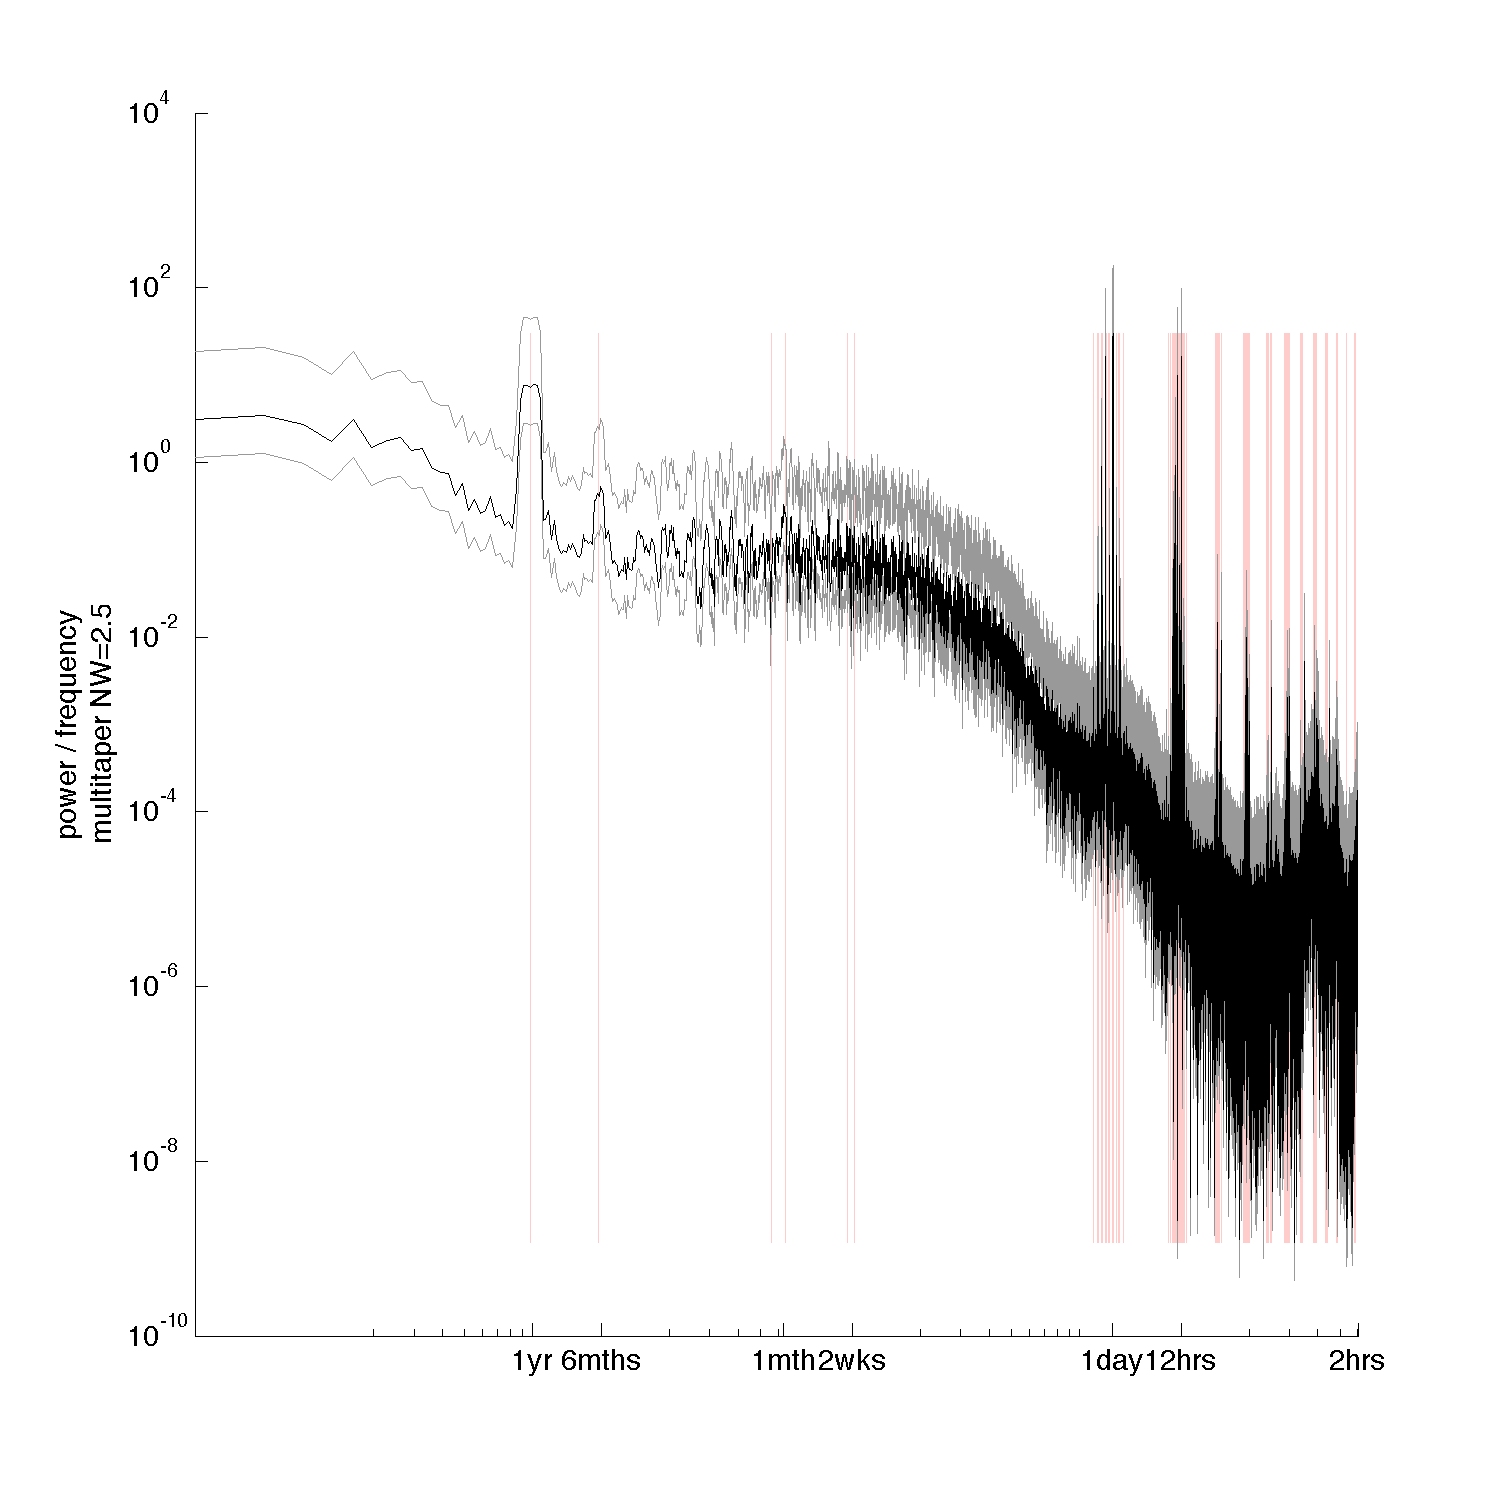
\includegraphics[width=\textwidth]{figures/plots/spectra_109504.png}
    \end{figure}
\end{minipage}
\hfill
\begin{minipage}{0.45\textwidth}
    \begin{figure}      
     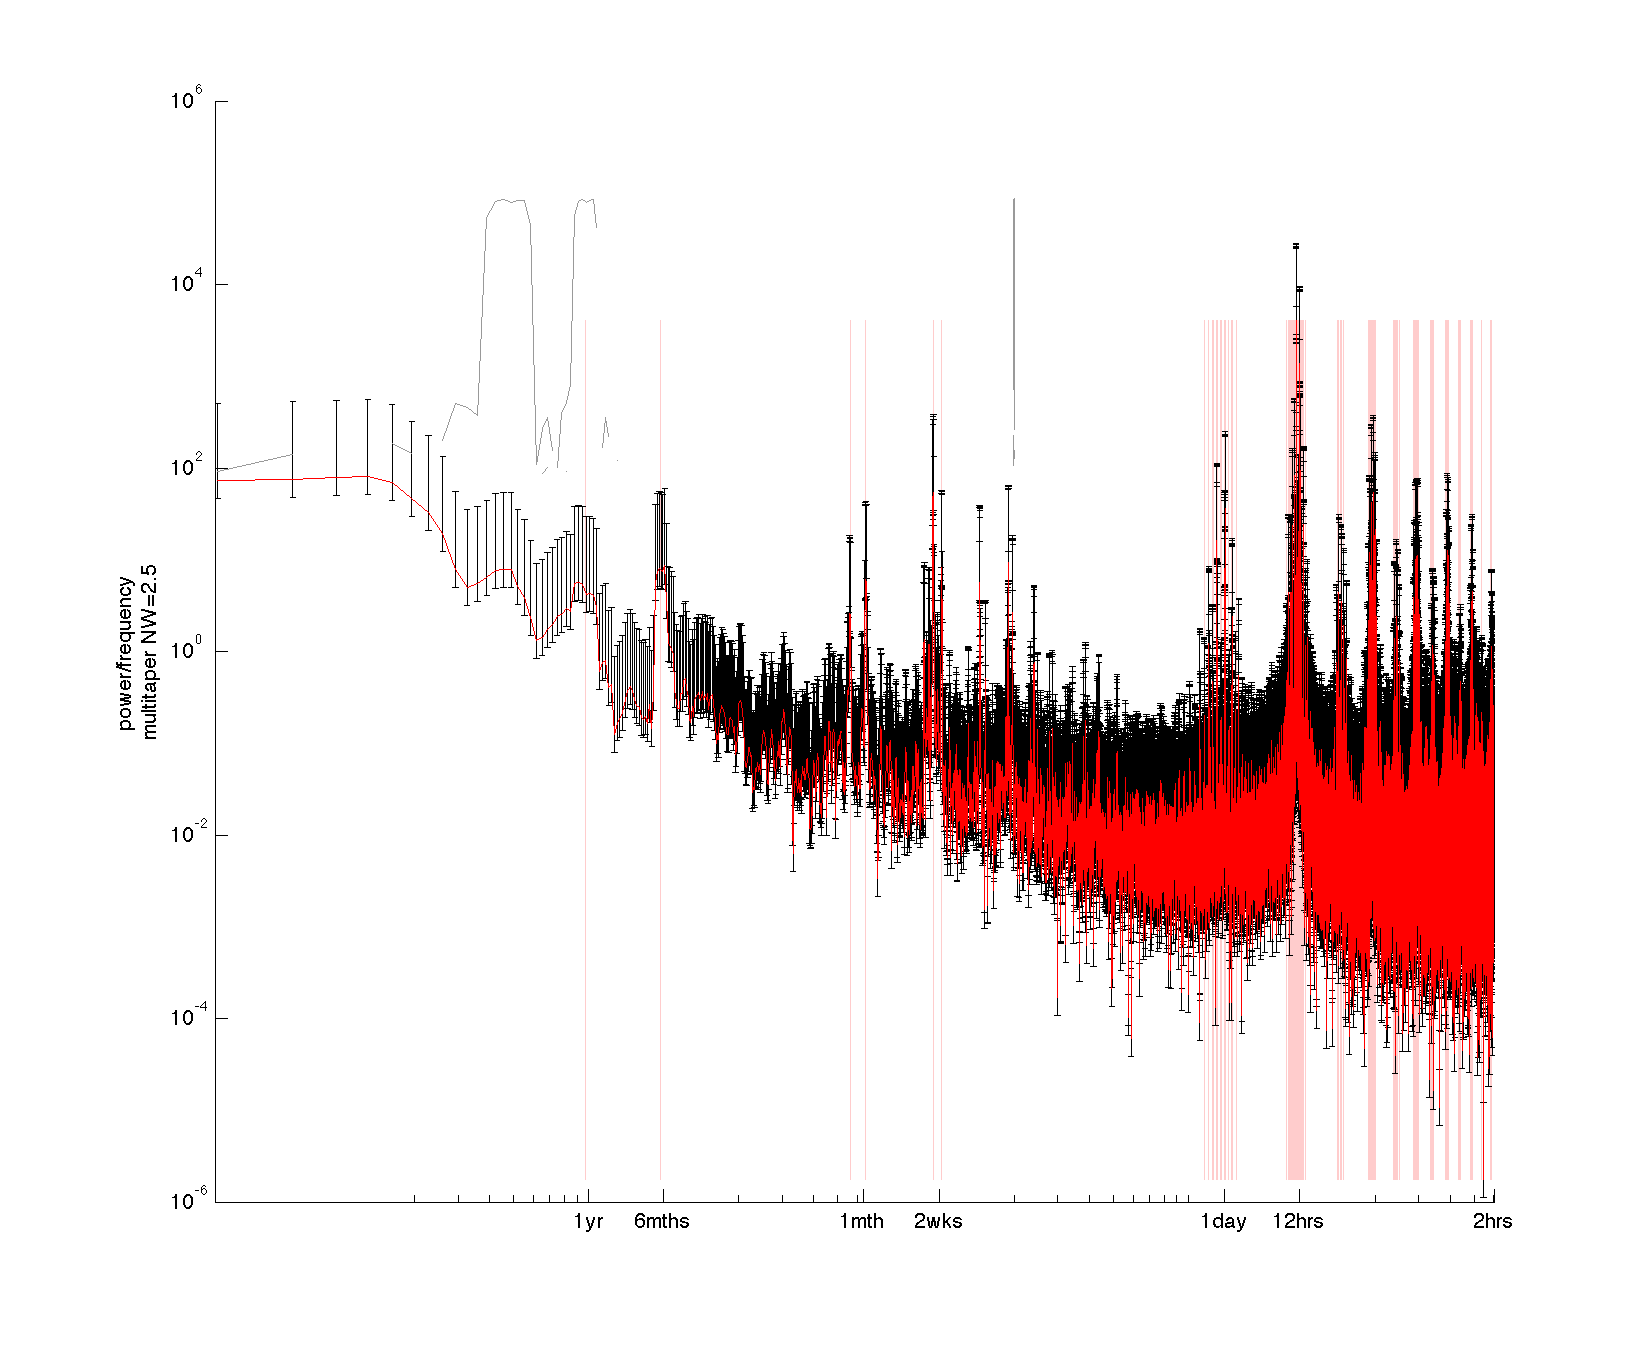
\includegraphics[width=\textwidth]{figures/plots/sealevel_spectra.png}
    \end{figure} 
\end{minipage}
\end{frame}
%-----------------------------------------
\begin{frame}
\frametitle{Forecast scales}
\begin{minipage}{0.45\textwidth}
    \begin{figure}      
    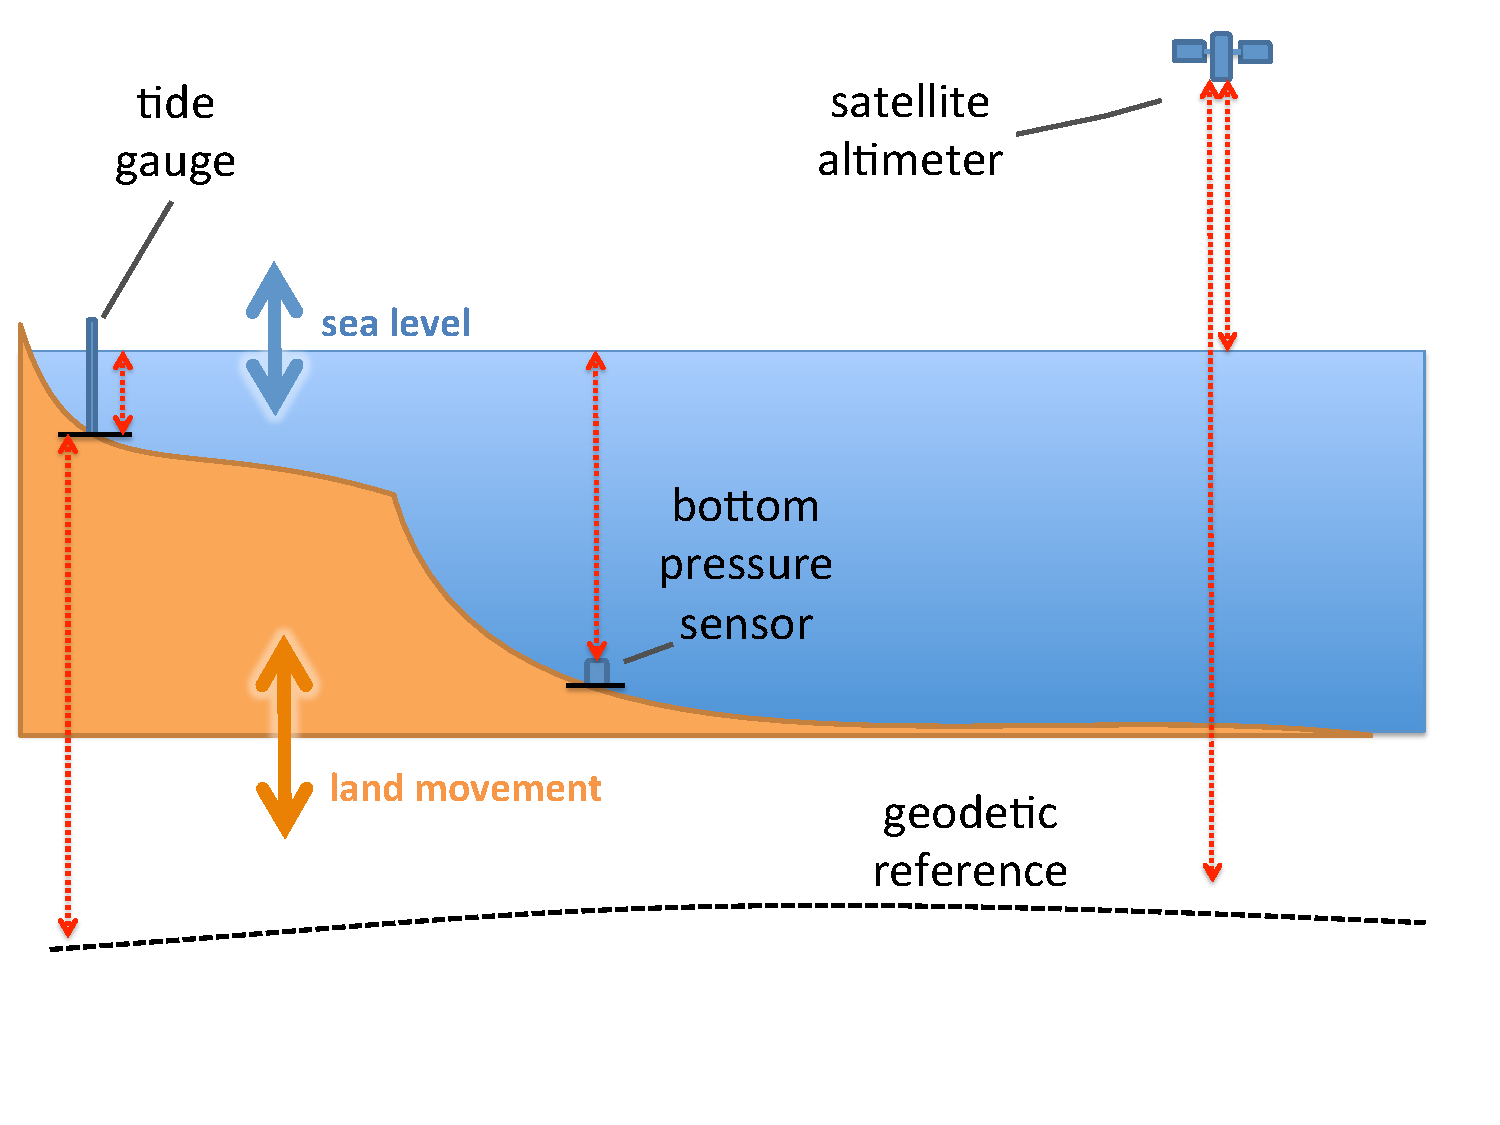
\includegraphics[width=\textwidth]{figures/diagrams/sealevel_cartoon.pdf}
    \end{figure}
\end{minipage}
\hfill
\begin{minipage}{0.45\textwidth}
    \begin{figure}      
     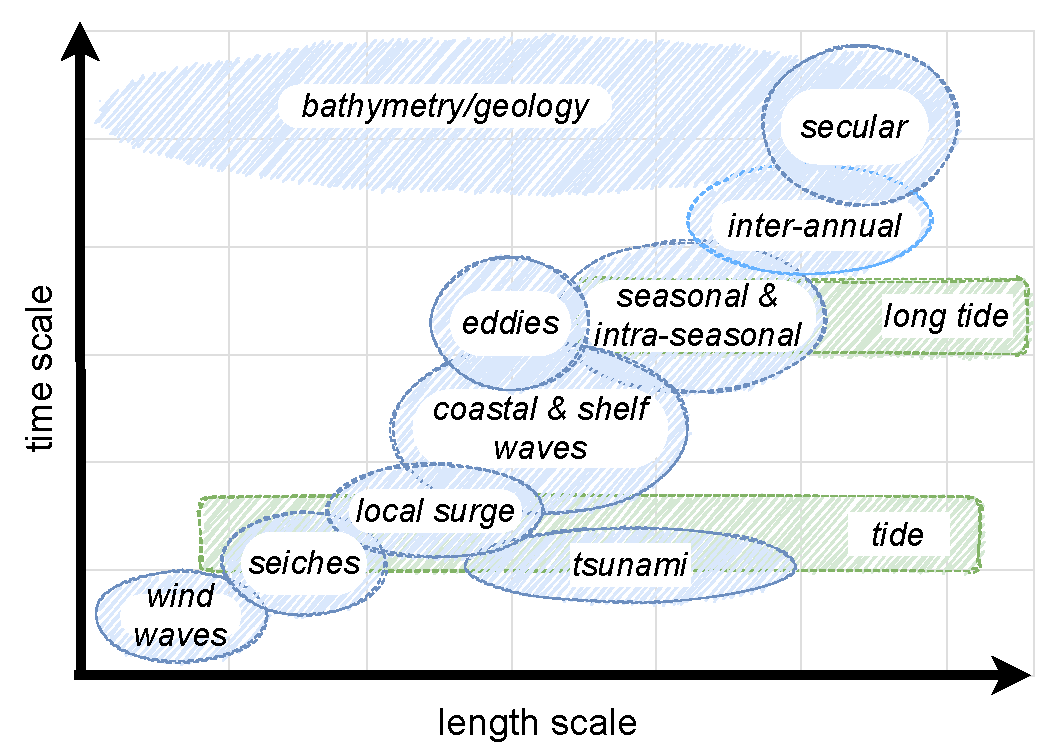
\includegraphics[width=\textwidth]{figures/diagrams/scales_time_length.pdf}
    \end{figure} 
\end{minipage}
\end{frame}
%-----------------------------------------
\begin{frame}
\frametitle{Tangible illustration of problem}
\centering
Useful in combination?\\
Need to wait for downscale for improvement?
\begin{minipage}{0.45\textwidth}
    \begin{figure}      
    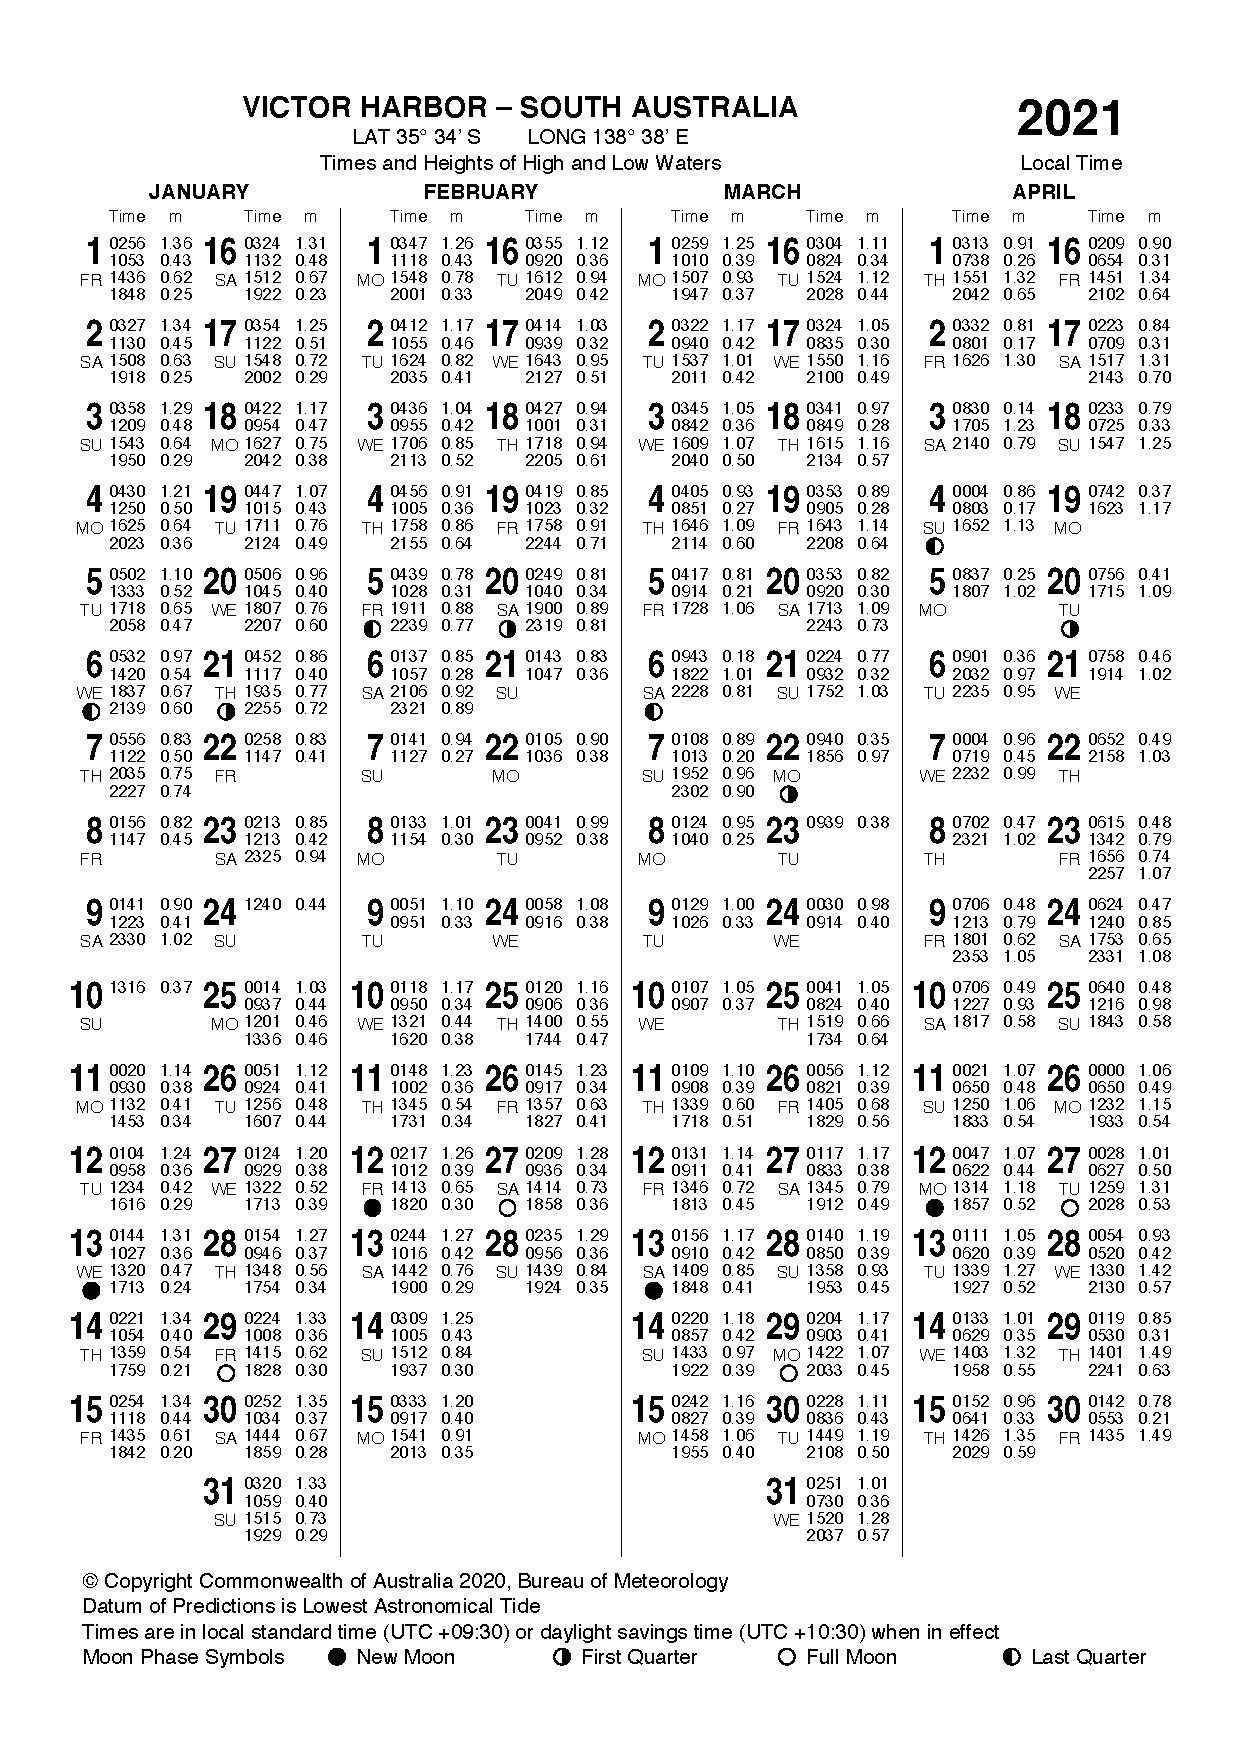
\includegraphics[trim={0 8cm 0 0},clip,height=\textheight]{figures/images/IDO59001_2021_SA_TP006.pdf}
    \end{figure}
\end{minipage}
\hfill
\begin{minipage}{0.45\textwidth}
    \begin{figure}      
     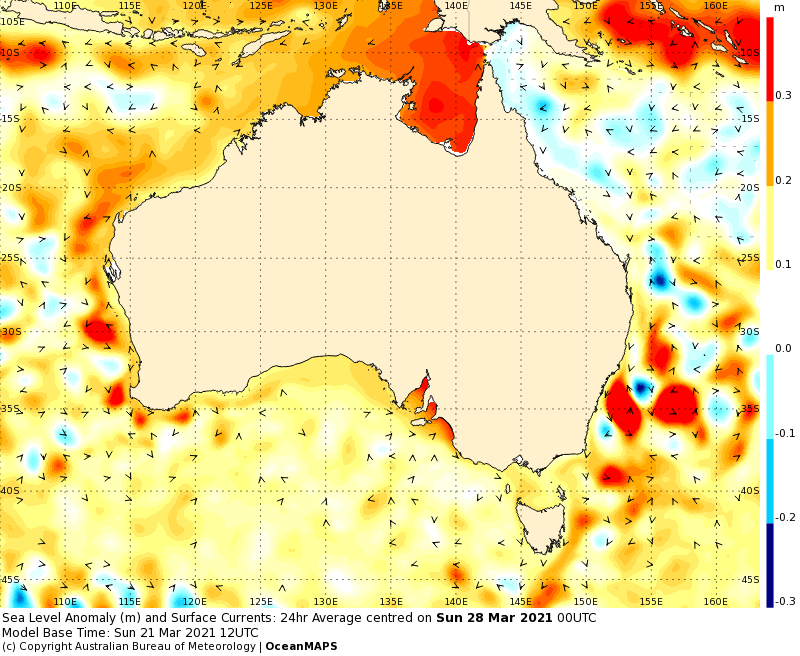
\includegraphics[width=\textwidth]{figures/images/IDYOC300.Aus.SLACur.168.png}
    \end{figure} 
\end{minipage}
\end{frame}
%-----------------------------------------
\begin{frame}
\frametitle{Tangible illustration of problem}
Longer forecast window versus detail.\\
Non-extreme management.\\
\begin{minipage}{0.4\textwidth}
    \begin{figure}      
    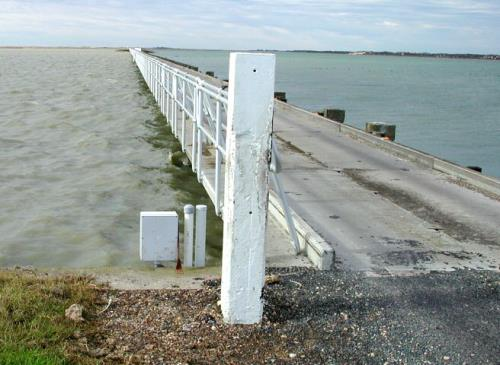
\includegraphics[height=0.4\textheight]{figures/images/goolwa_ewe_island-environment_sa_gov_au.jpg}
    \end{figure}
\end{minipage}
\hfill
\begin{minipage}{0.4\textwidth}
    \centering
     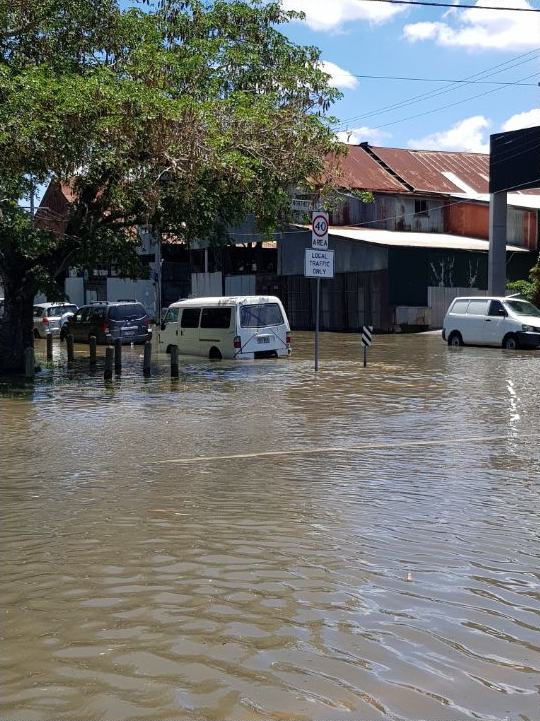
\includegraphics[width=0.8\textwidth]{figures/images/sunnyFlood_ClarkJan2018Brisbane.png} 
\end{minipage}

\end{frame}
%-----------------------------------------
\begin{frame}
\frametitle{Tangible illustration of problem}

\begin{minipage}{0.6\textwidth} 
\centering
      sea level and positioning\\
      
      
      tidal planes for elevation\\
      
      
      standard tides as reference\\
      
      
      boundary conditions, down-scaling
\end{minipage}
\begin{minipage}{0.3\textwidth}
    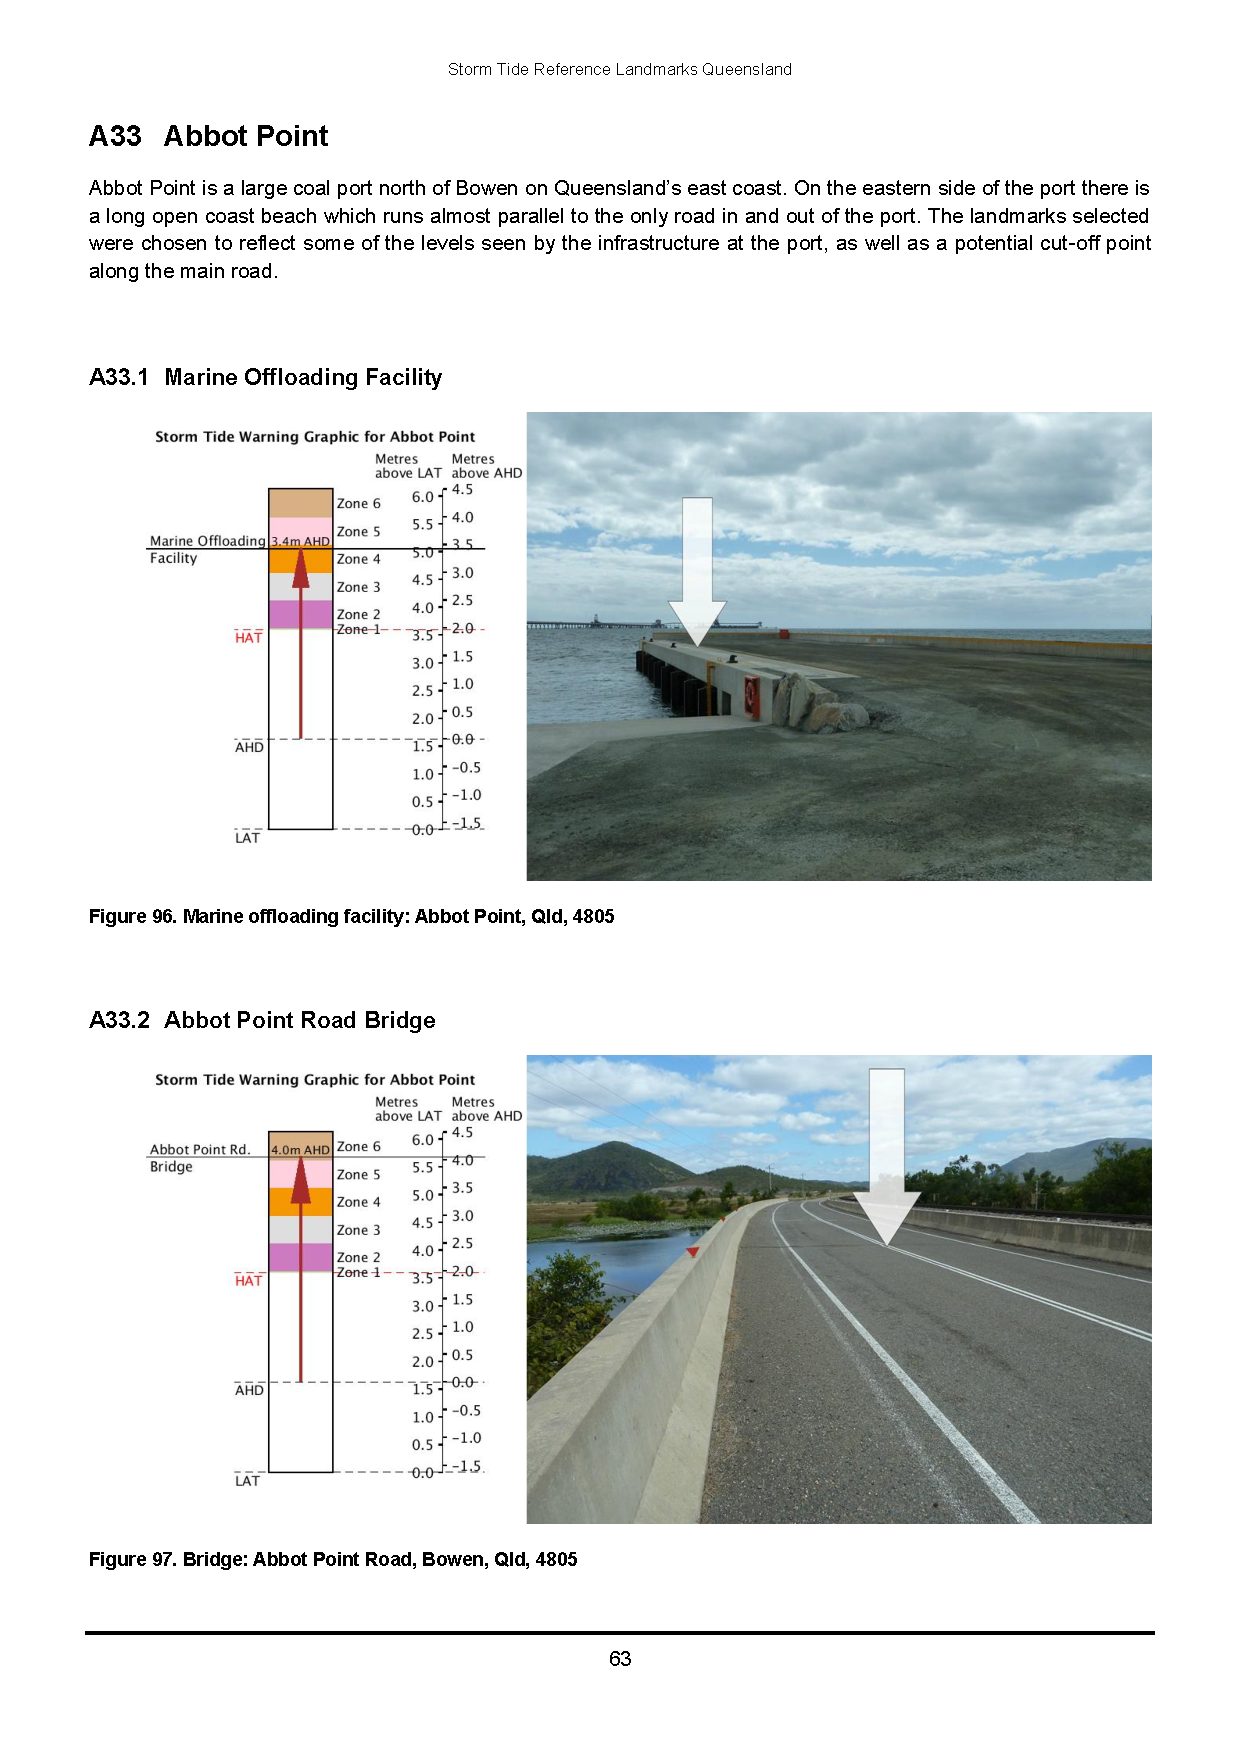
\includegraphics[trim={2cm 0 5cm 5cm},clip,height=0.9\textheight]{figures/images/qldLandmarkEg.pdf}
\end{minipage}

\end{frame}


%--------
\section{Sea level forecast concepts}
\begin{frame}
\frametitle{Historical context}

Tides and forecasting
analysis 
tide tables
laws and convention


NWP
satellites
godae
altimeters
data assimilation


satellites
tides 
orbits
corrections


government
'official'
references
services

\end{frame}
%-----------------------------------------
\begin{frame}
\frametitle{Motivating applications}
\begin{minipage}{0.45\textwidth}
    \begin{figure}      
    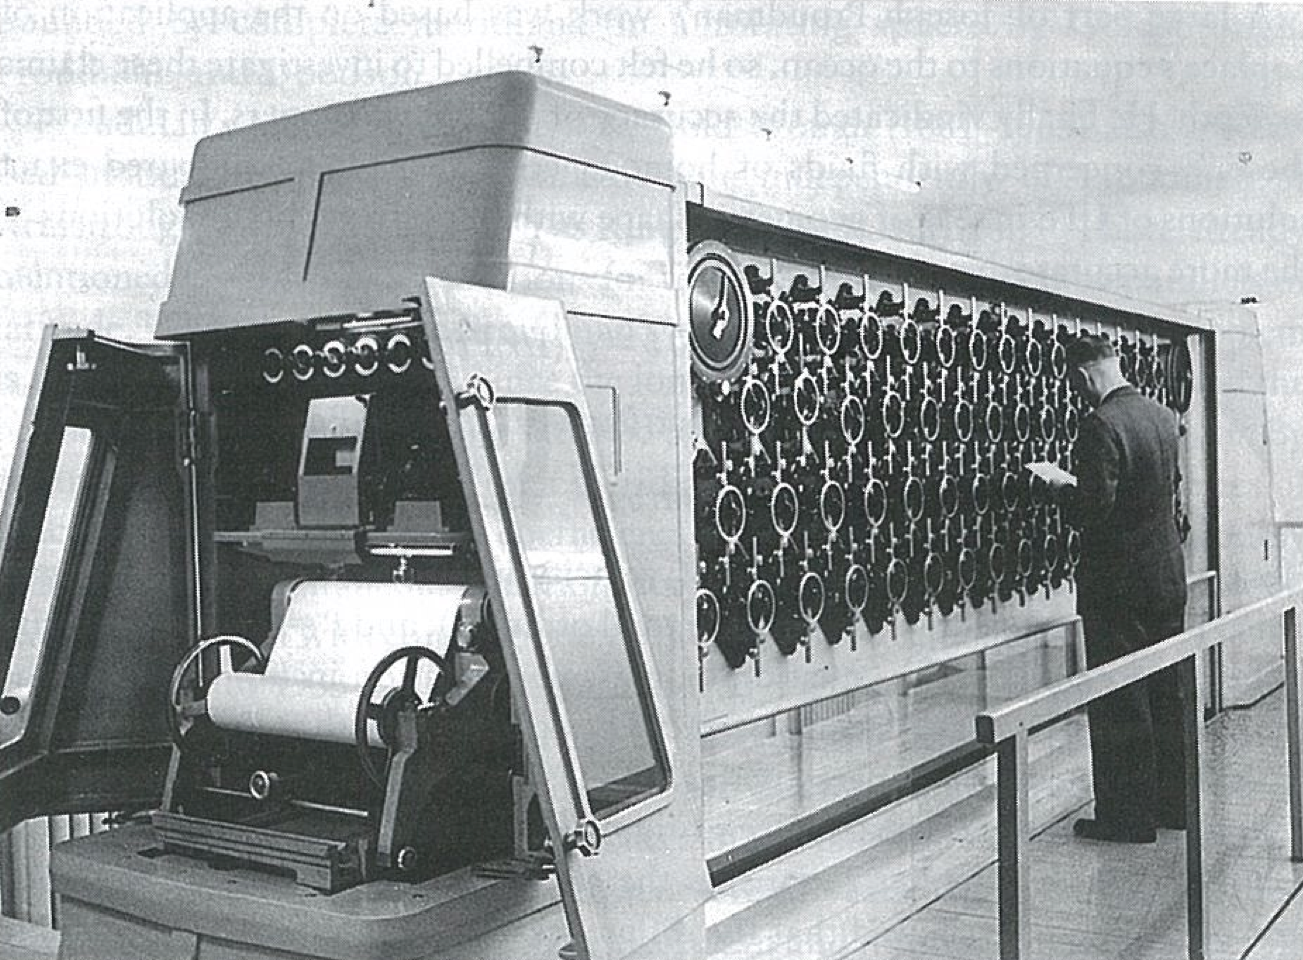
\includegraphics[width=\textwidth]{figures/images/DHI_machine_cartwright_fig11p2.png}
    \end{figure}
\end{minipage}
\hfill
\begin{minipage}{0.45\textwidth}
    Some text here.
\end{minipage}
\end{frame}
%-----------------------------------------
%--------
\section{(1)Direct aggregation with mesoscale forecast}
%-----------------------------------------
\begin{frame}
\frametitle{Immediate simplest hybrid - direct aggregation}
    \begin{figure}      
    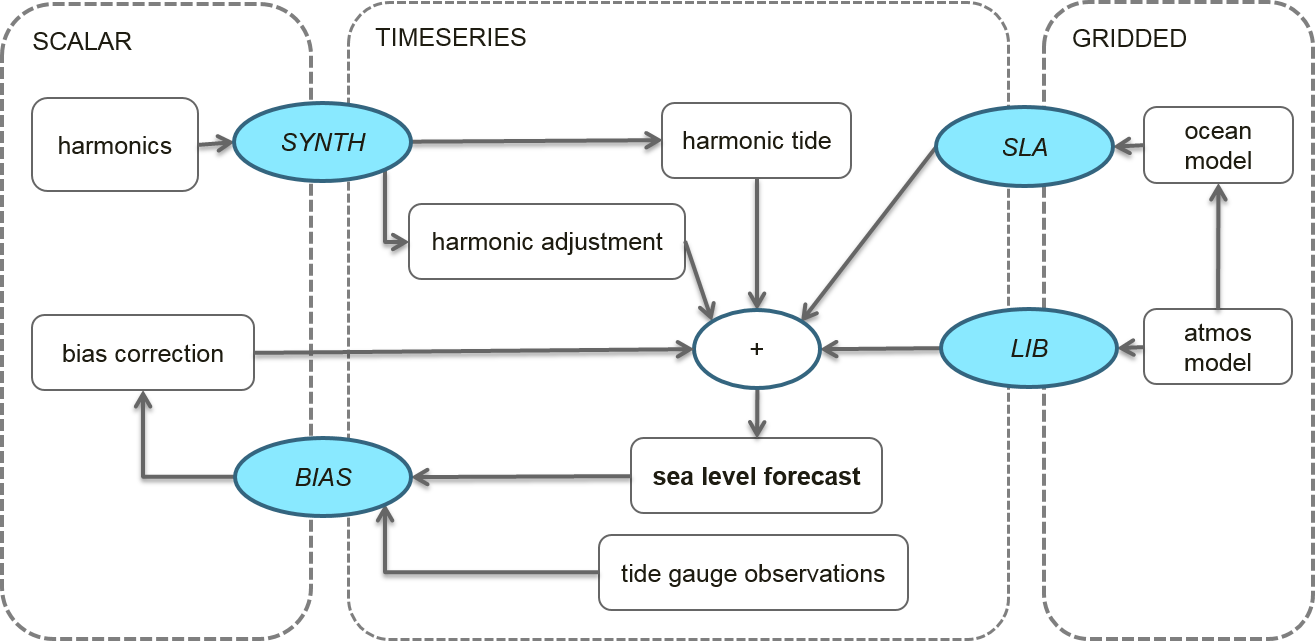
\includegraphics[width=\textwidth]{figures/diagrams/aggSL_schematic_abstract.png}
    \end{figure}
\end{frame}
%-----------------------------------------
\begin{frame}
\frametitle{Immediate simplest hybrid - direct aggregation}
    \begin{figure}      
    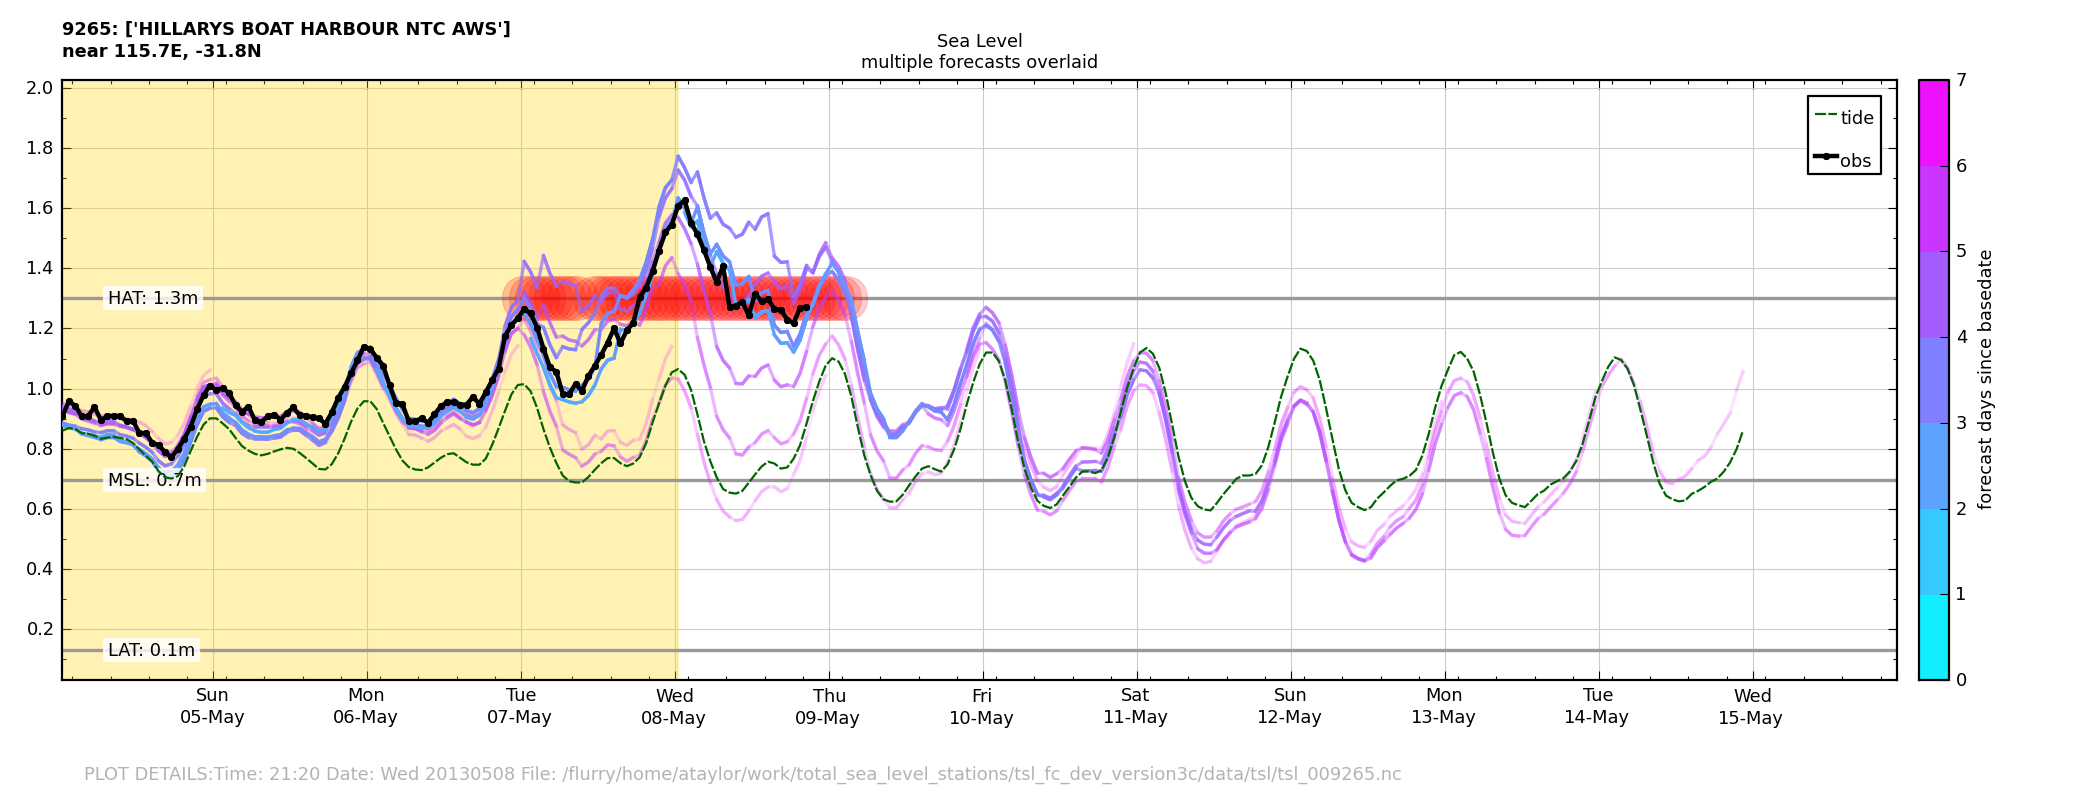
\includegraphics[width=\textwidth]{figures/plots/aggregate_fc_plot_009265.png}
    \end{figure}
\end{frame}
%-----------------------------------------
\begin{frame}
\frametitle{Spatial scales}
    \begin{figure}      
    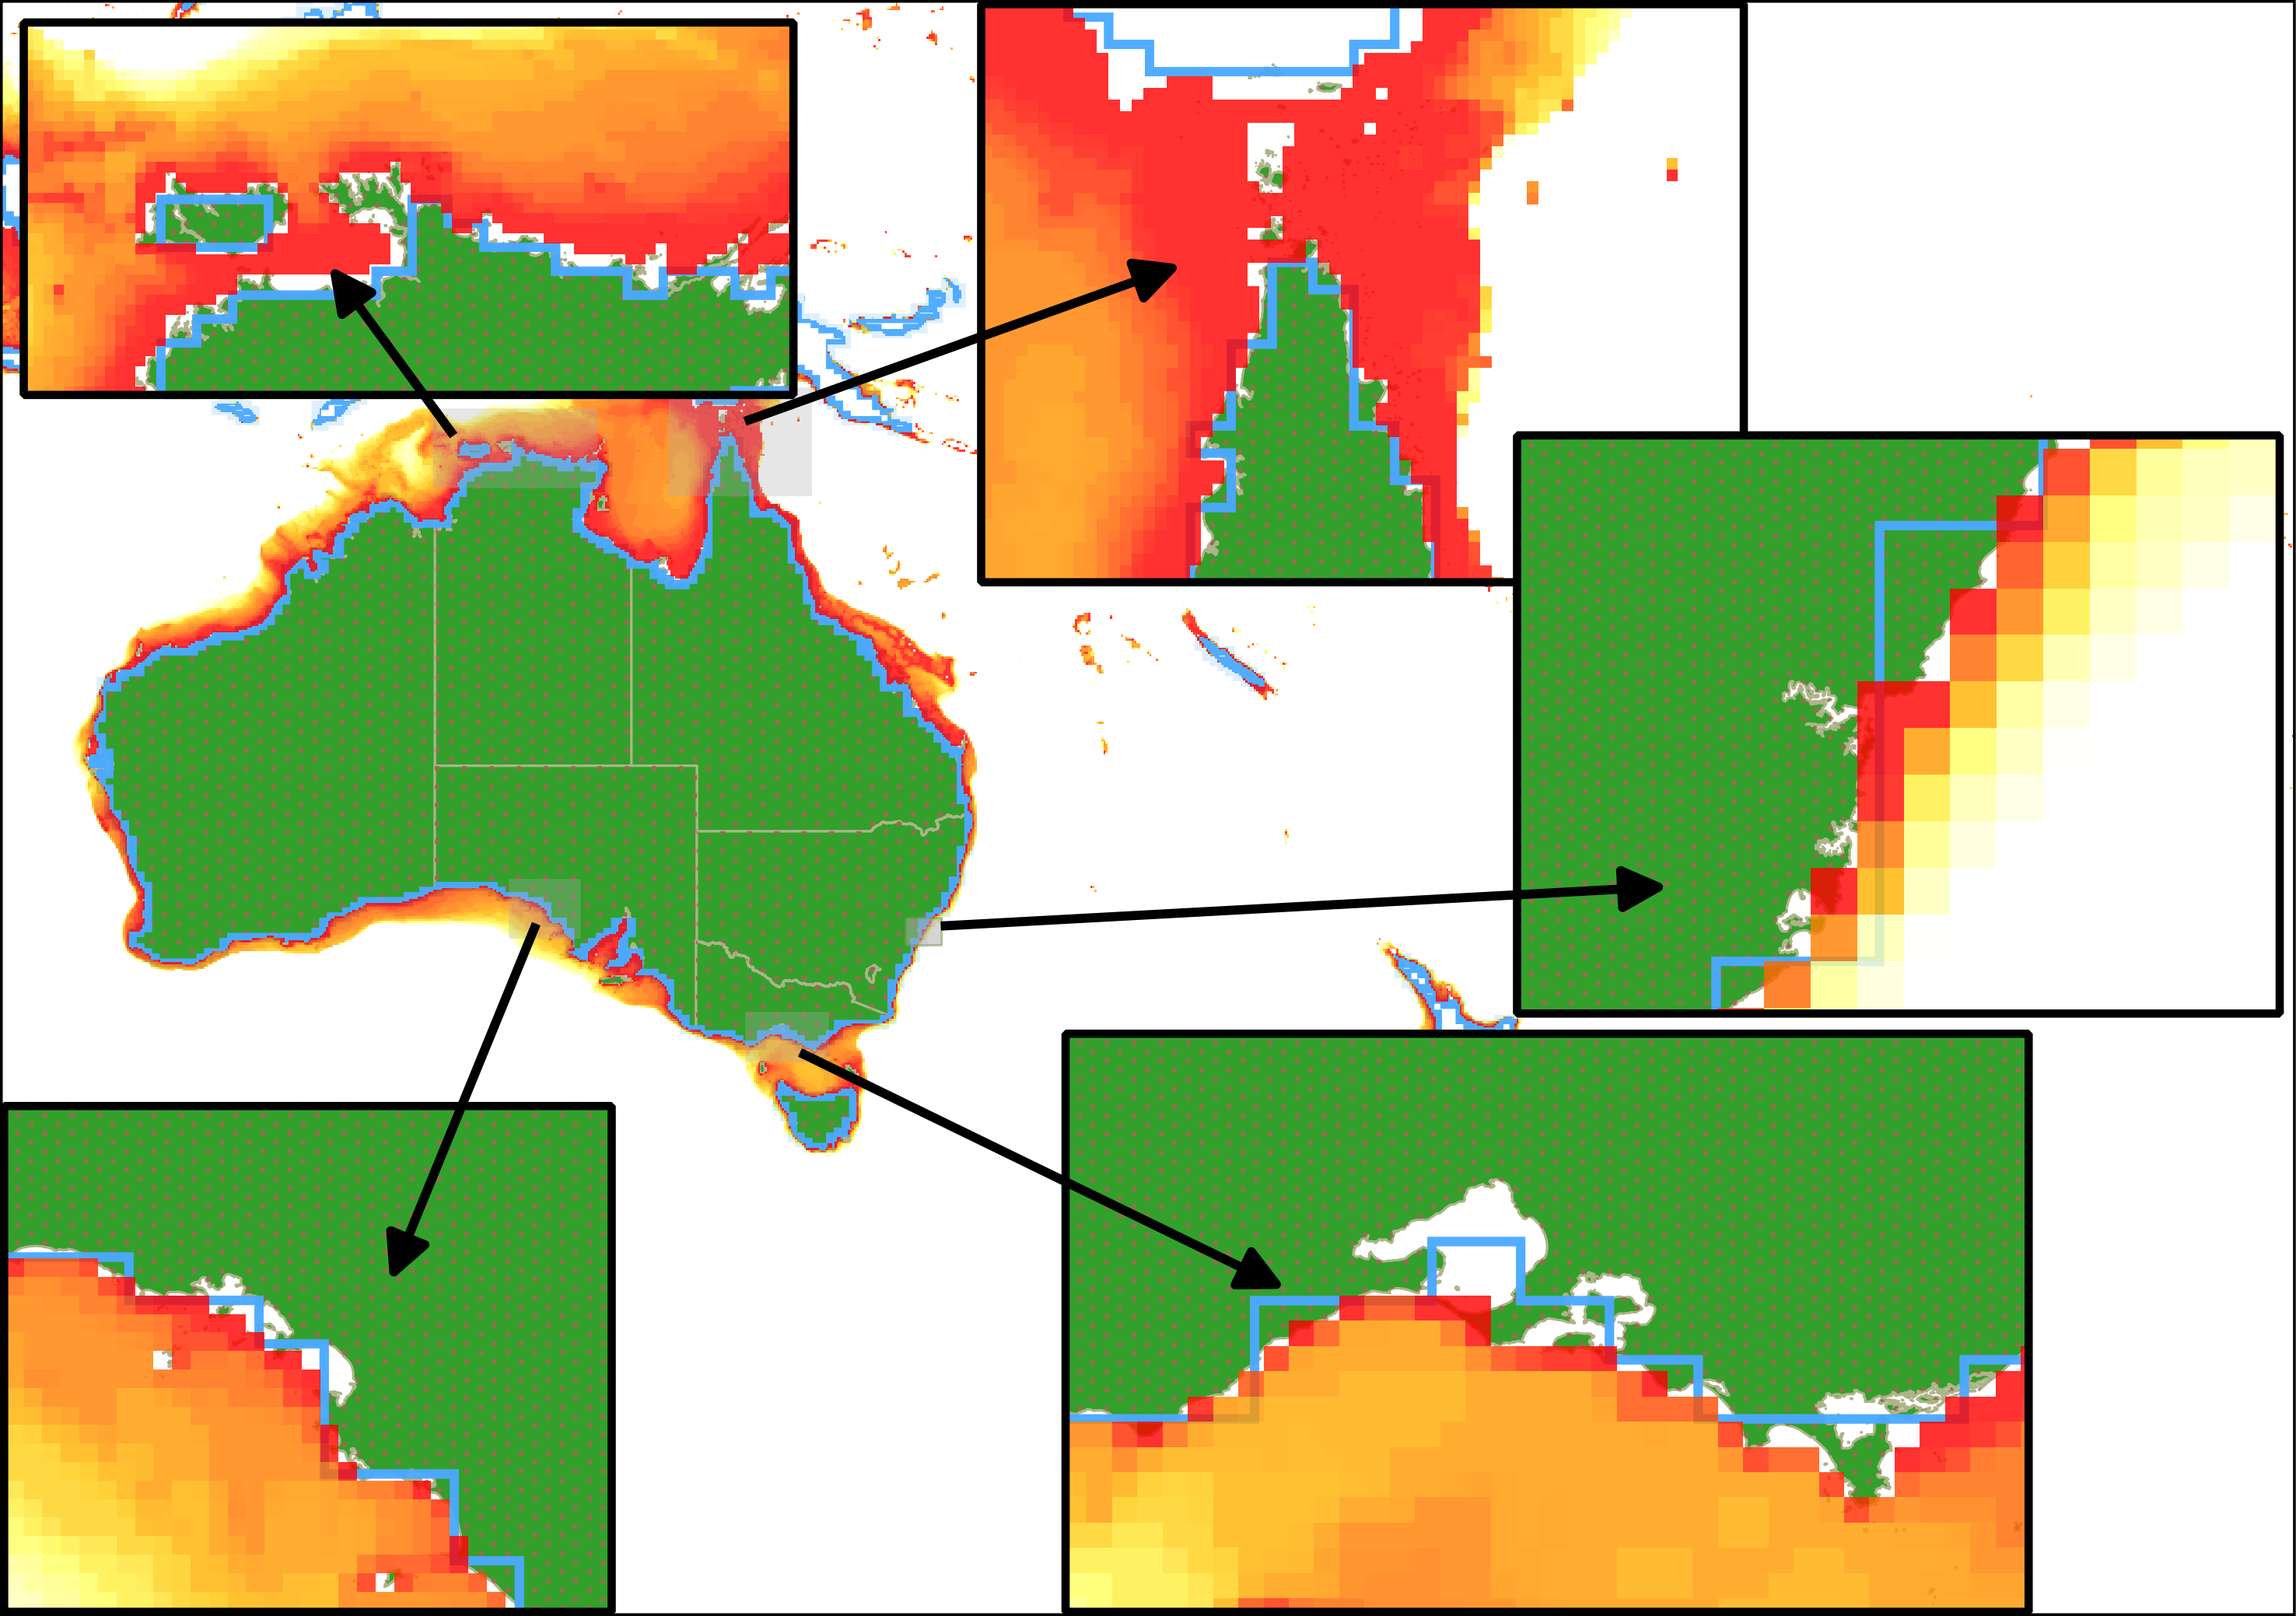
\includegraphics[width=\textwidth]{figures/maps/omaps_masks.png}
    \end{figure}
\end{frame}
%-----------------------------------------
\begin{frame}
\frametitle{characterise spatial skill}
    \begin{figure}      
    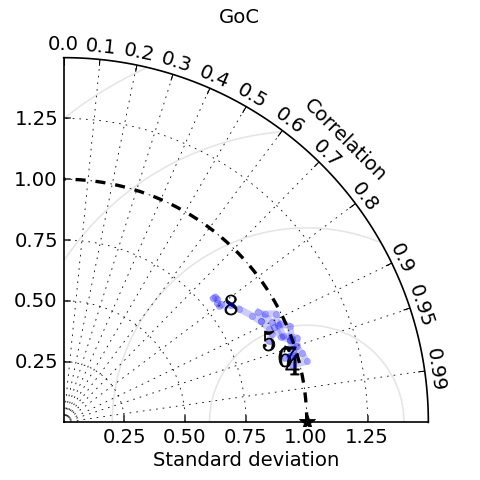
\includegraphics[width=0.3\textwidth]{figures/plots/taylor_diag_res_GoC.png}
    \end{figure}
\end{frame}
%-----------------------------------------
\begin{frame}
\frametitle{bias term}
\begin{figure}      
    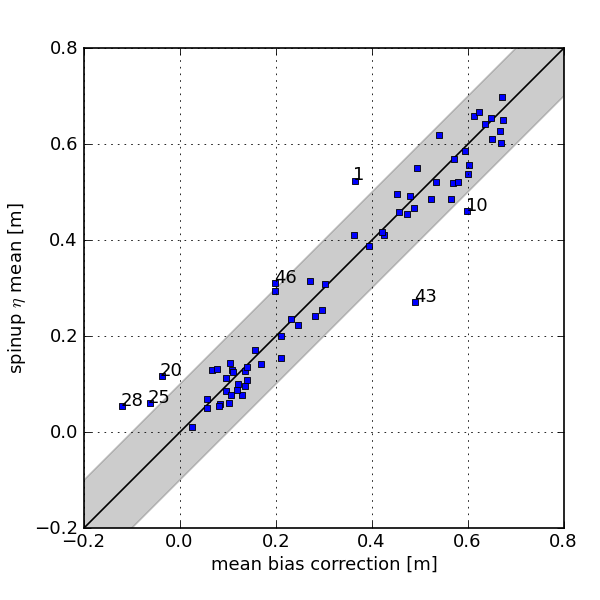
\includegraphics[width=0.3\textwidth]{figures/plots/aggSL_bias_breakdown_plot_1.png}
    \end{figure}
\end{frame}
%-----------------------------------------
\begin{frame}
\frametitle{harmonic tide adjustment}
\end{frame}
%-----------------------------------------
%\begin{frame}
%\frametitle{tbc}
%\begin{minipage}{0.45\textwidth}
%    \begin{figure}      
%    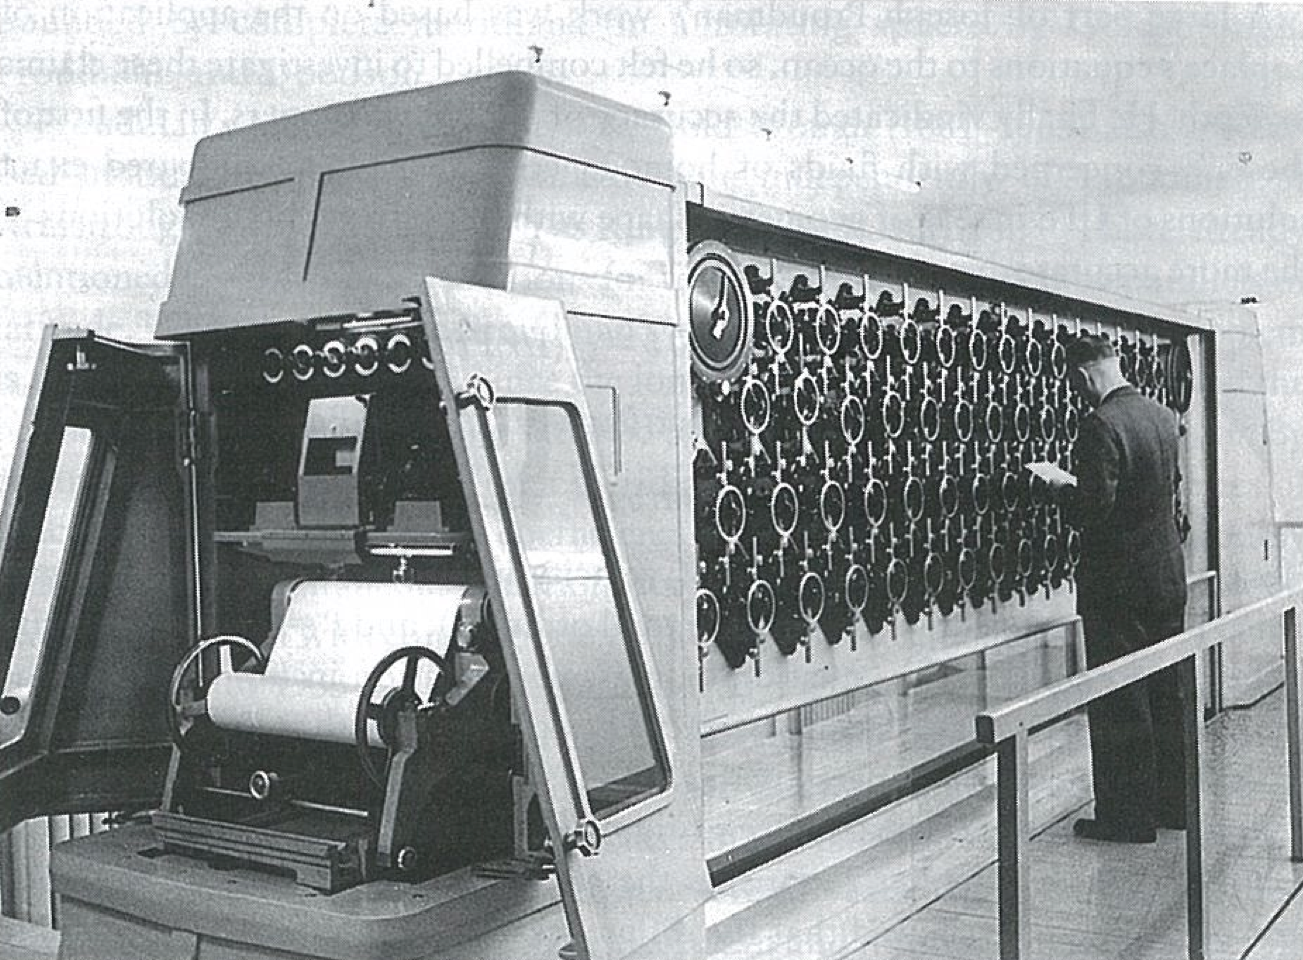
\includegraphics[width=\textwidth]{figures/images/DHI_machine_cartwright_fig11p2.png}
%    \end{figure}
%\end{minipage}
%\hfill
%\begin{minipage}{0.45\textwidth}
%    \begin{figure}      
%    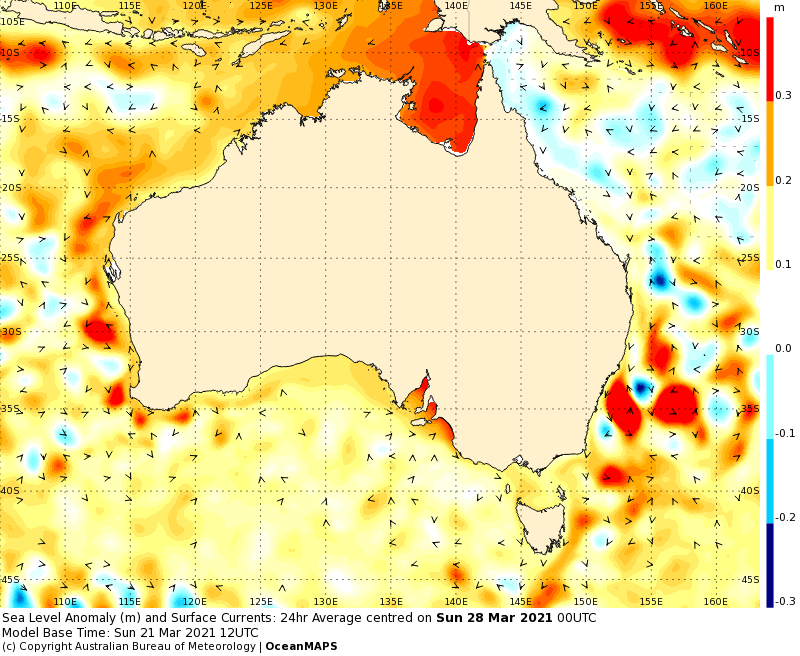
\includegraphics[width=\textwidth]{figures/images/IDYOC300.Aus.SLACur.168.png}
%    \end{figure}
%\end{minipage}
%\end{frame}
%--------
\section{(2) Value of a coastal waveguide view}
%-----------------------------------------
\begin{frame}
\frametitle{Coastal waveguide view}
\begin{columns}
    \begin{column}{0.5\textwidth}
      \centering
      framework for aggregation\\
      targeted evaluation \\
      guidance and `narrative'\\
      analogy with atmosphere equatorial\\
      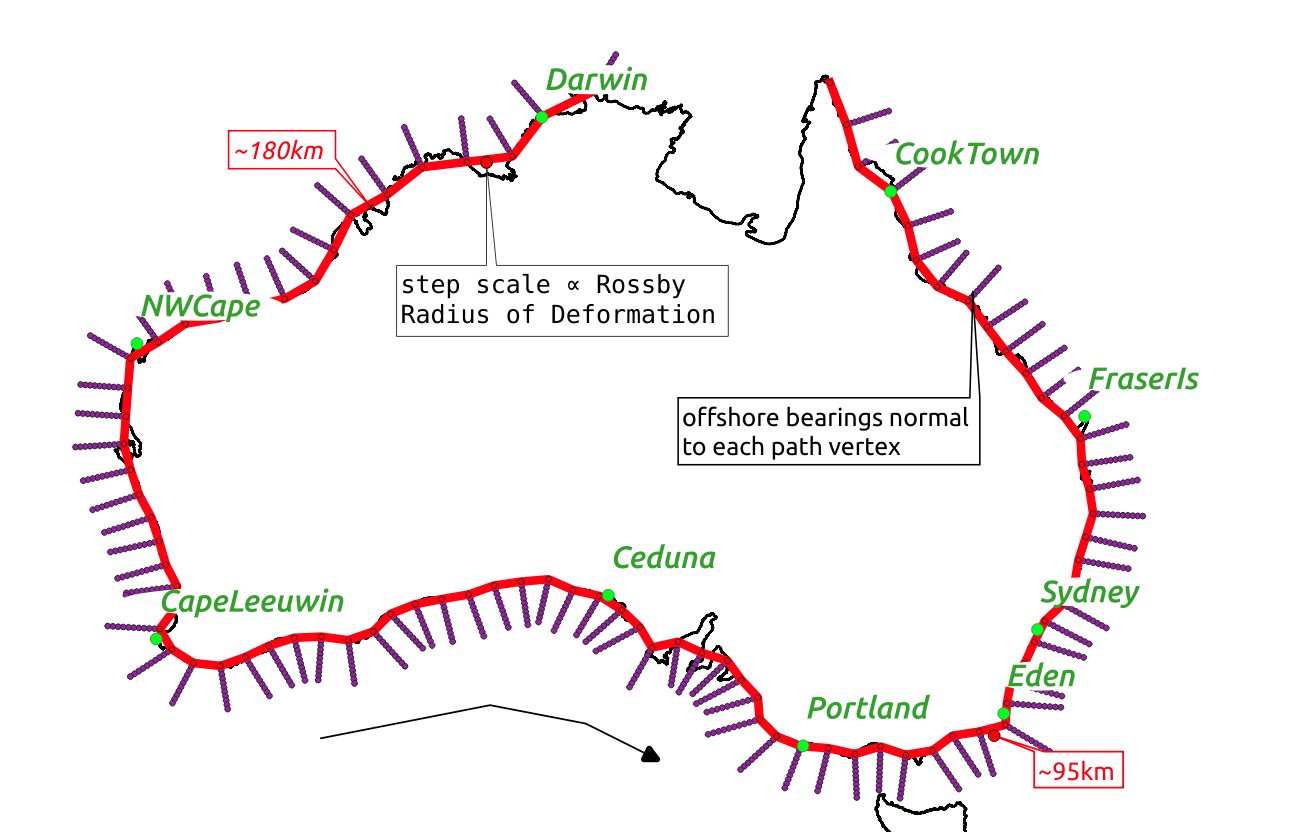
\includegraphics[width=\textwidth]{figures/maps/map_overview.png}
    \end{column}

    \begin{column}{0.5\textwidth}
        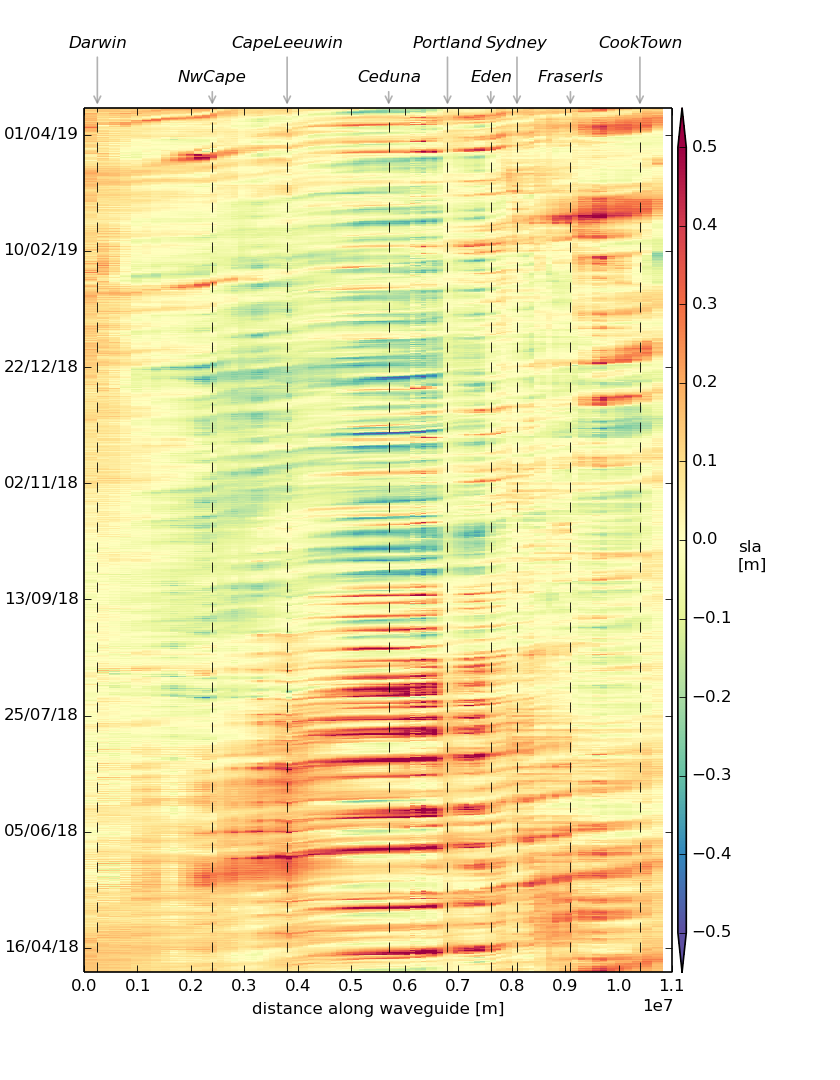
\includegraphics[width=\textwidth]{figures/plots/concat_sla_day0_full.png}
    \end{column}
\end{columns}
\end{frame}
%-----------------------------------------
\begin{frame}
\frametitle{How long is that path?}
    quantitative comparison of celerity
    resolution explicit\\
    but not model dependant
    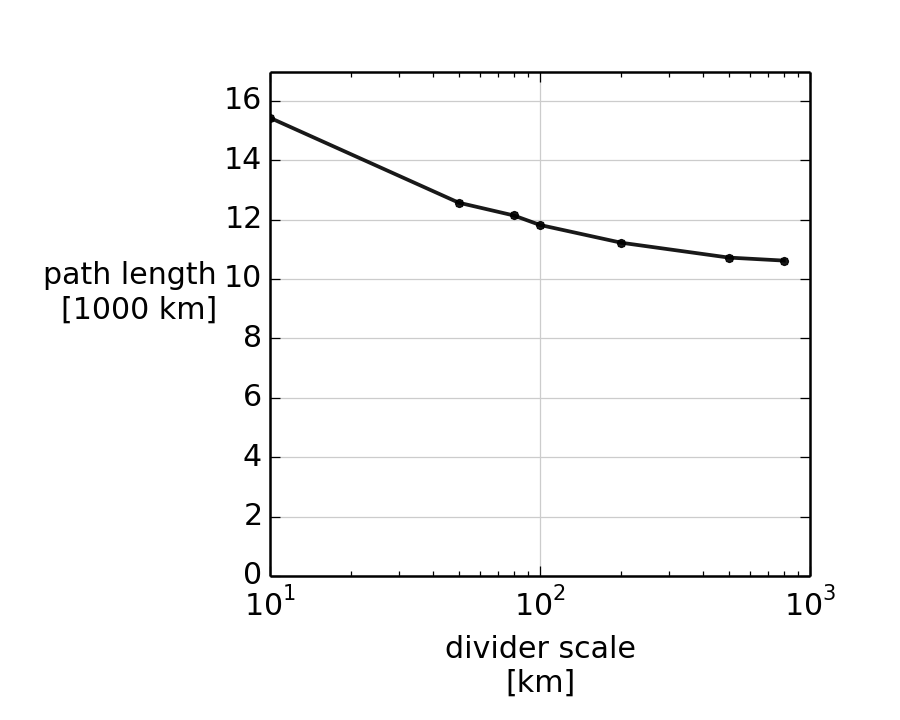
\includegraphics[height=0.6\textheight]{figures/plots/mandelbrot_lengths.png}
\end{frame}
%-----------------------------------------
\begin{frame}
\frametitle{Tides, double counting and adjustments}
ensuring tidal component is fit-for-purpose\\
blunt allocation of constituent cause as "non astromical"\\
conceptual barriers in operations\\
\vfill{}
    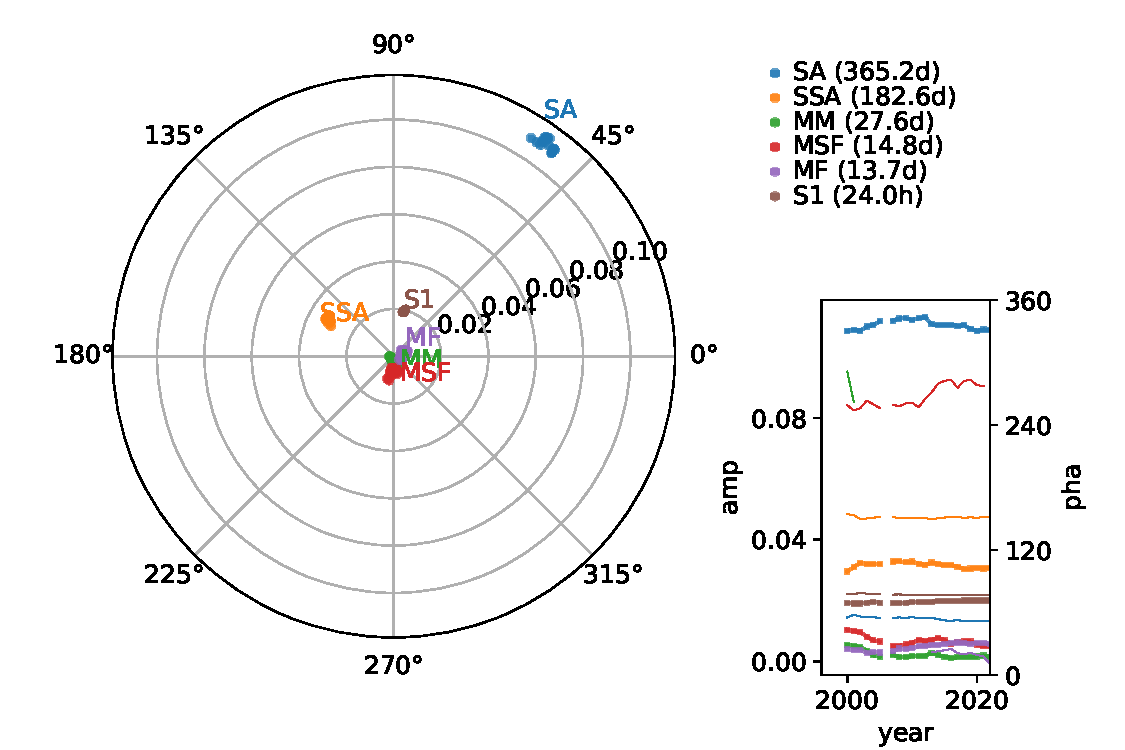
\includegraphics[width=0.45\textwidth]{figures/plots/complex_62290.pdf}
    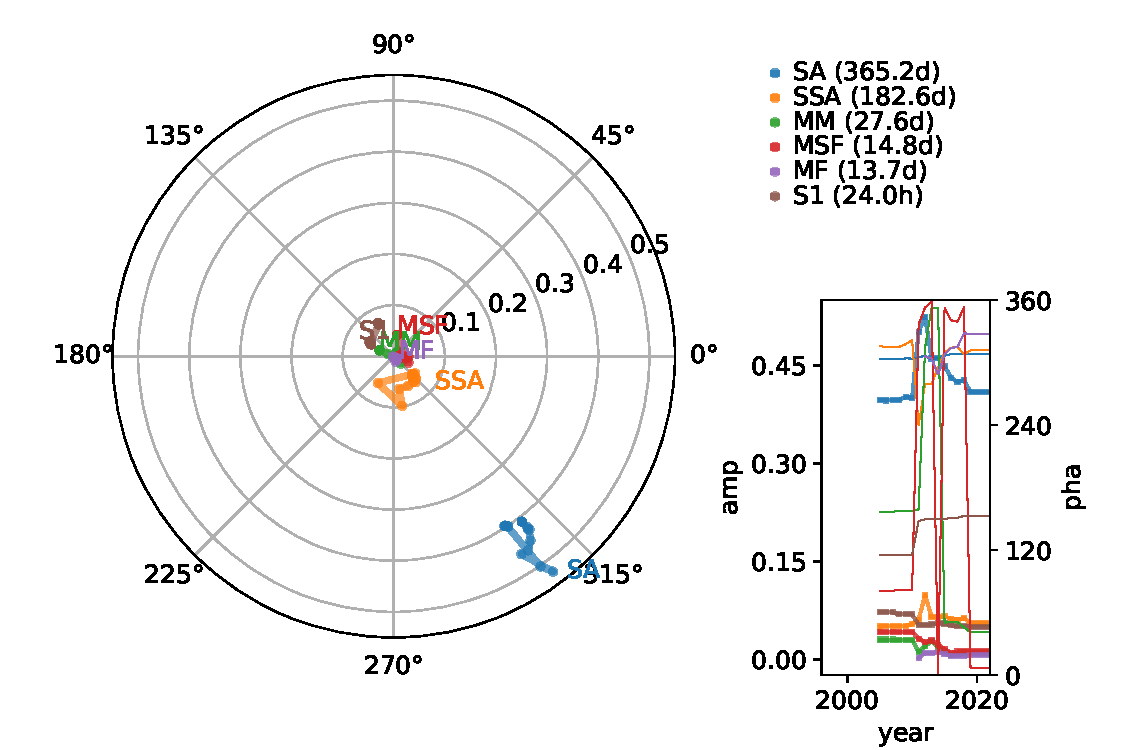
\includegraphics[width=0.45\textwidth]{figures/plots/complex_63540.pdf}
\end{frame}


%--------
\section{(3) Adapting a conventional tide service}
%-----------------------------------------
\begin{frame}
\frametitle{Tidal systems in operations}

\begin{minipage}{0.45\textwidth}
    \begin{figure}      
    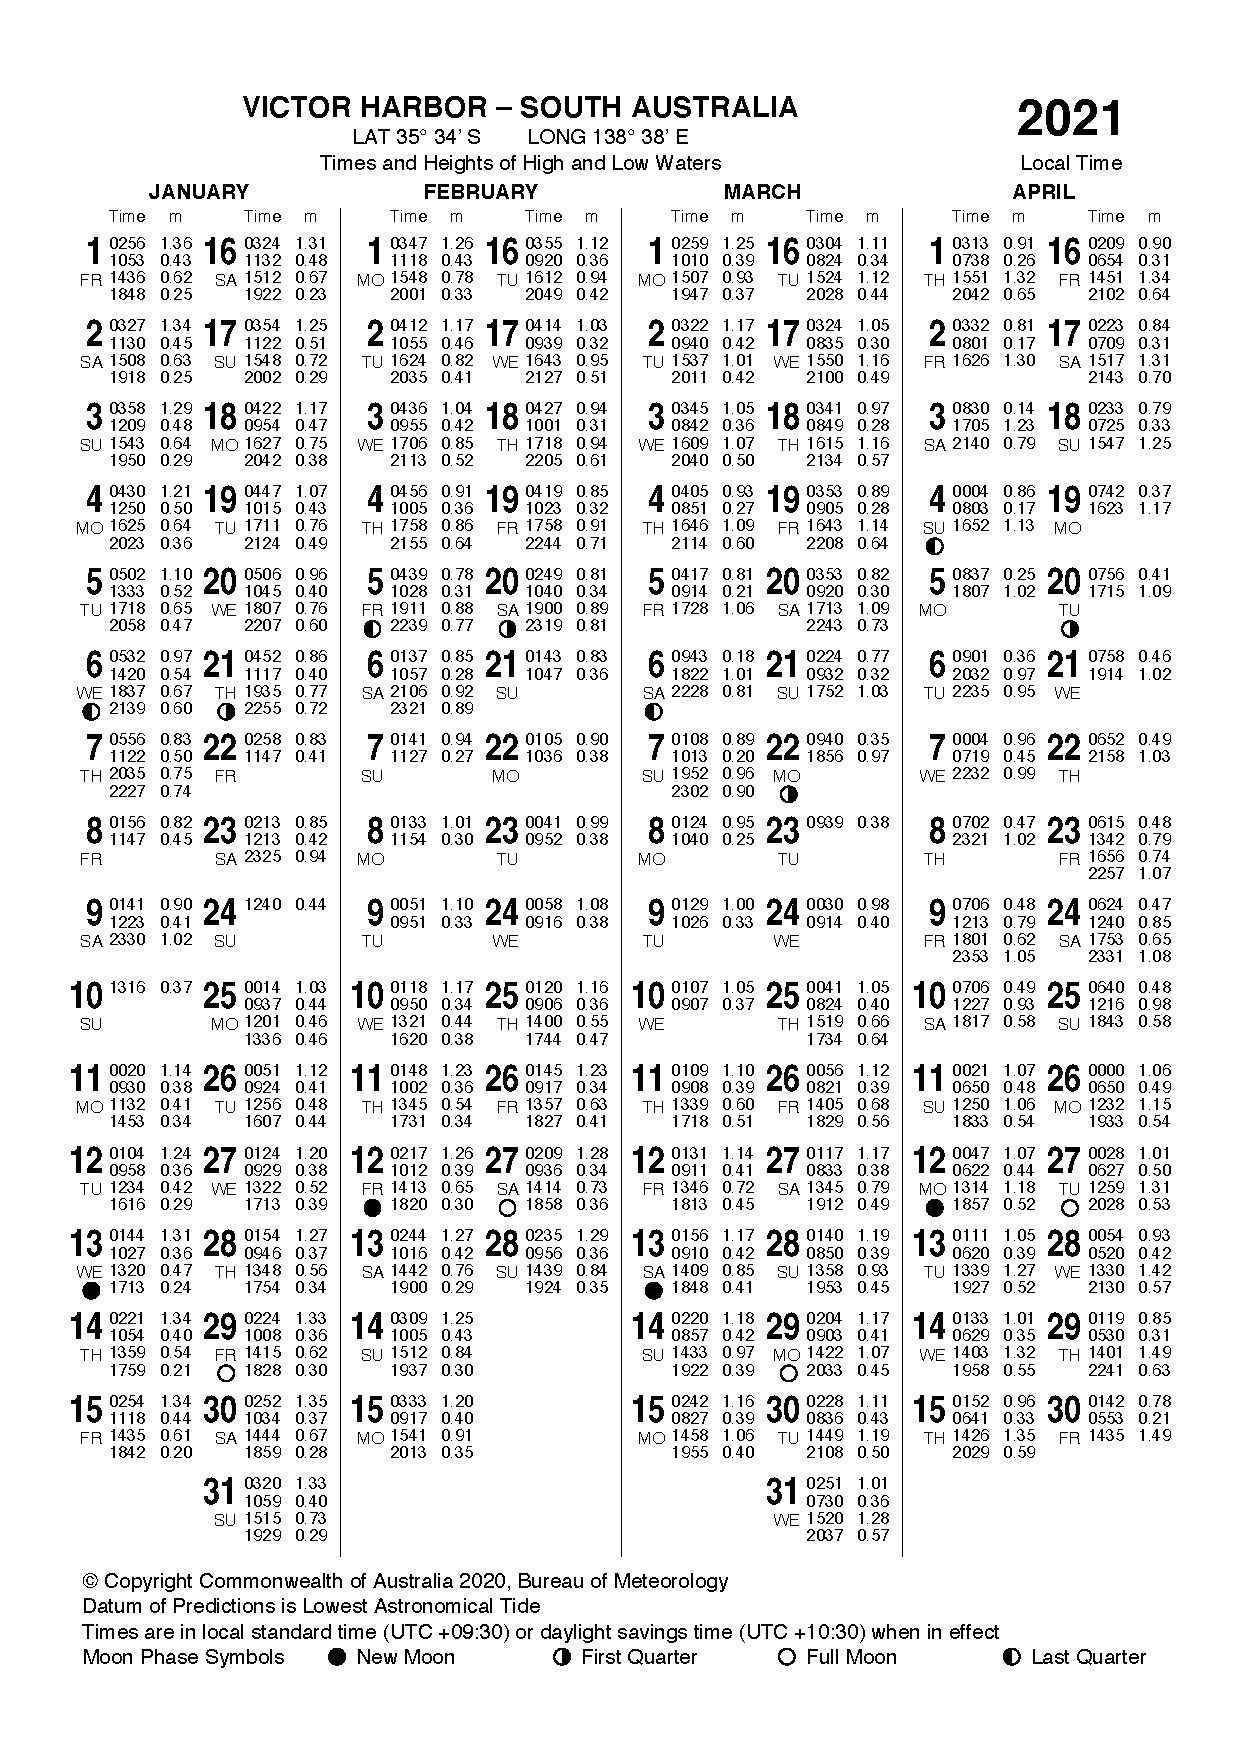
\includegraphics[height=0.4\textheight]{figures/images/IDO59001_2021_SA_TP006.pdf}
    \end{figure}
    forecast and filter?
    tsunami, 
\end{minipage}

\hfill

\begin{minipage}{0.45\textwidth}
    \begin{figure}      
     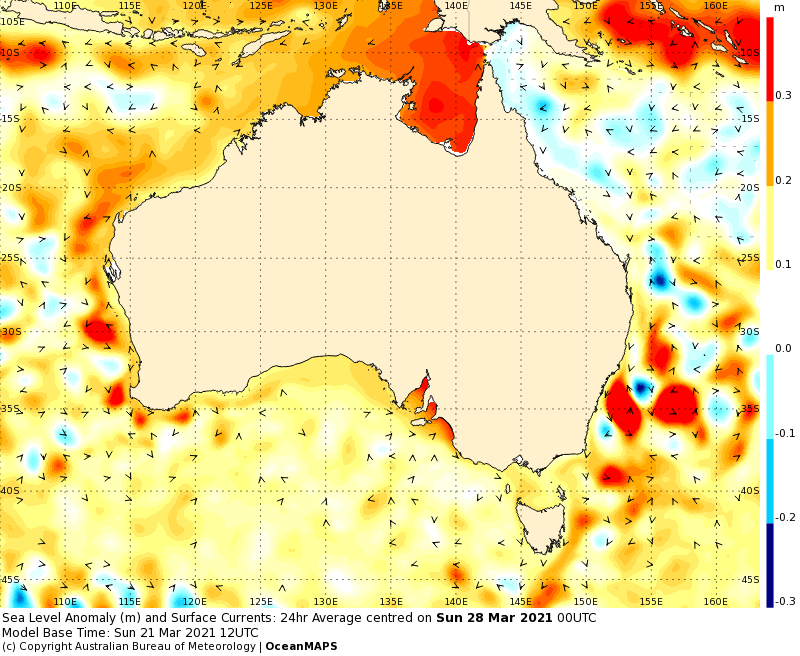
\includegraphics[width=\textwidth]{figures/images/IDYOC300.Aus.SLACur.168.png}
    \end{figure}
    altimeters - corrections
\end{minipage}


\end{frame}
%-----------------------------------------
\begin{frame}
\frametitle{Forecasts, physics, filters}

      \begin{figure}      
        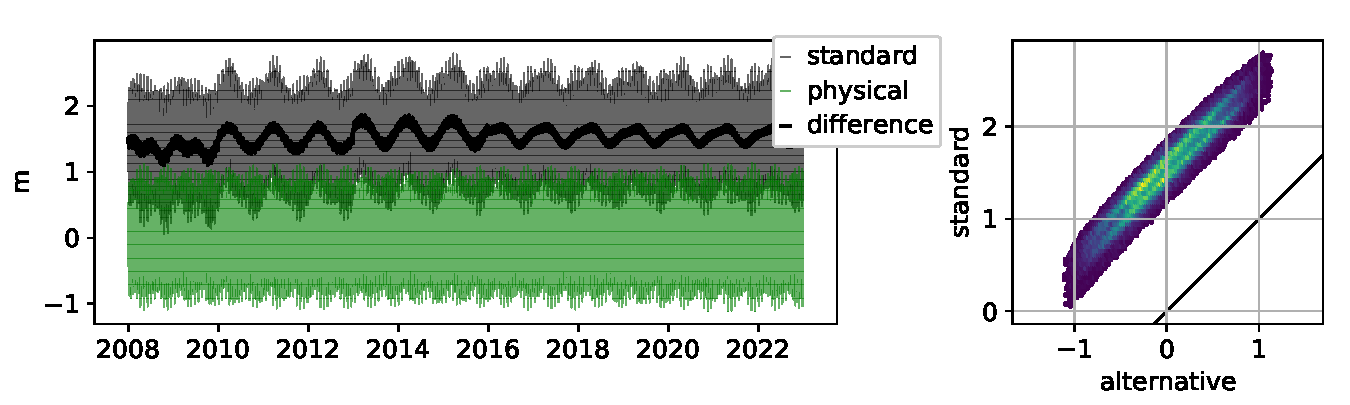
\includegraphics[width=\textwidth]{figures/plots/piecewiseTide_62430.pdf}
      \end{figure}

      \begin{itemize}
          \item standard annual tables - discontinuous
          \item contrast purpose and context
      \end{itemize}

\end{frame}
%-----------------------------------------
\begin{frame}
\frametitle{Global versus ``standard'' tides}
\begin{columns}
    \begin{column}{0.7\textwidth}
      \begin{figure}      
        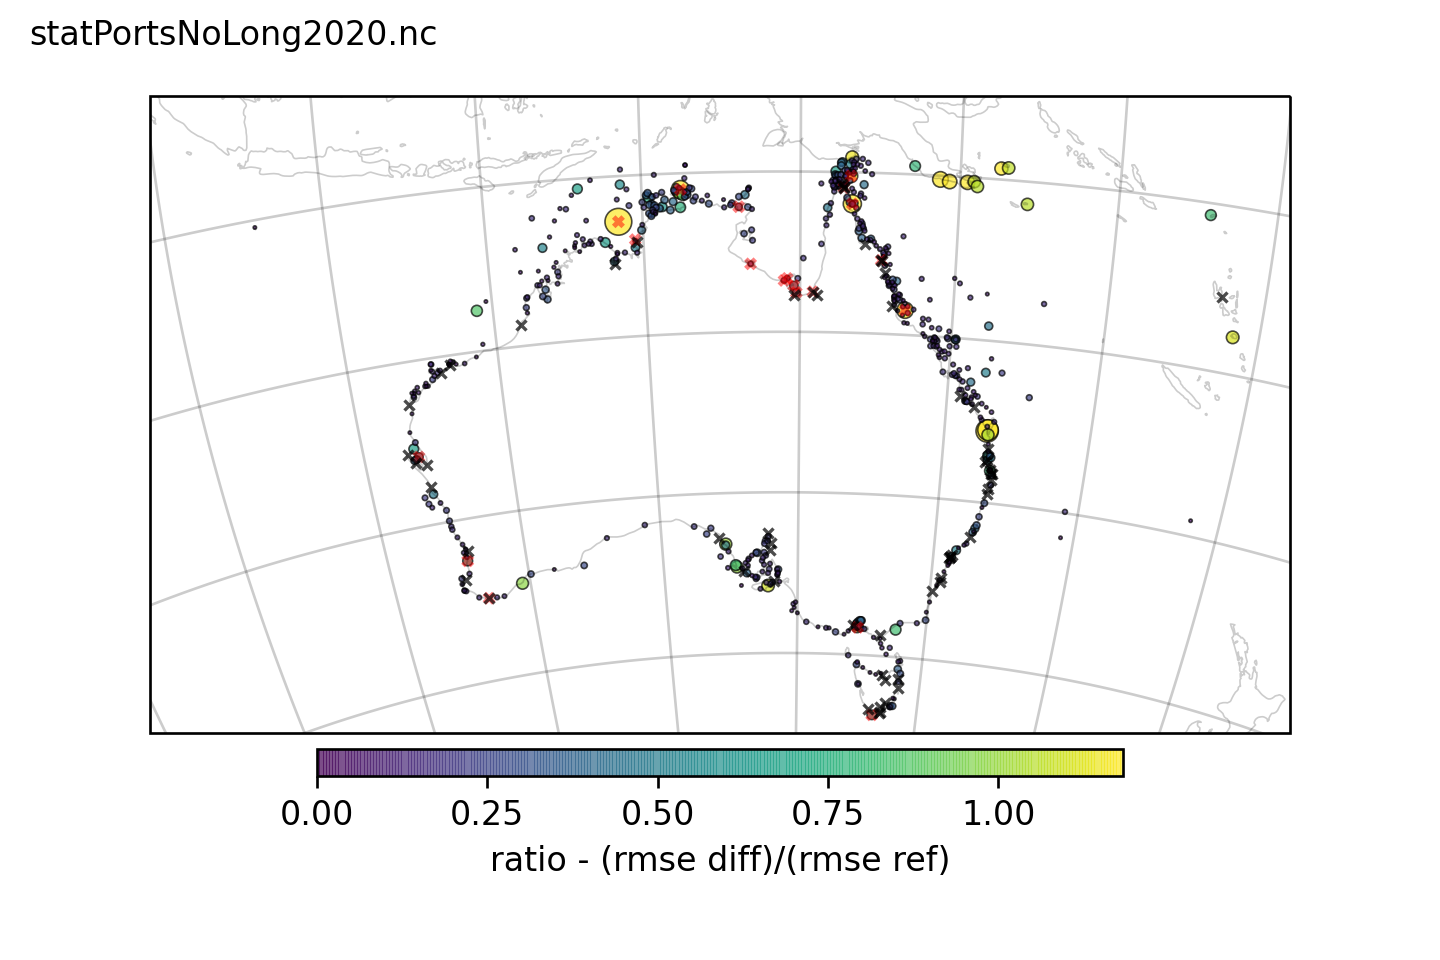
\includegraphics[width=\textwidth]{figures/maps/portsdiffRmseRatioNoLong.png}
      \end{figure}
    \end{column}

    \begin{column}{0.3\textwidth}
      \begin{figure}      
        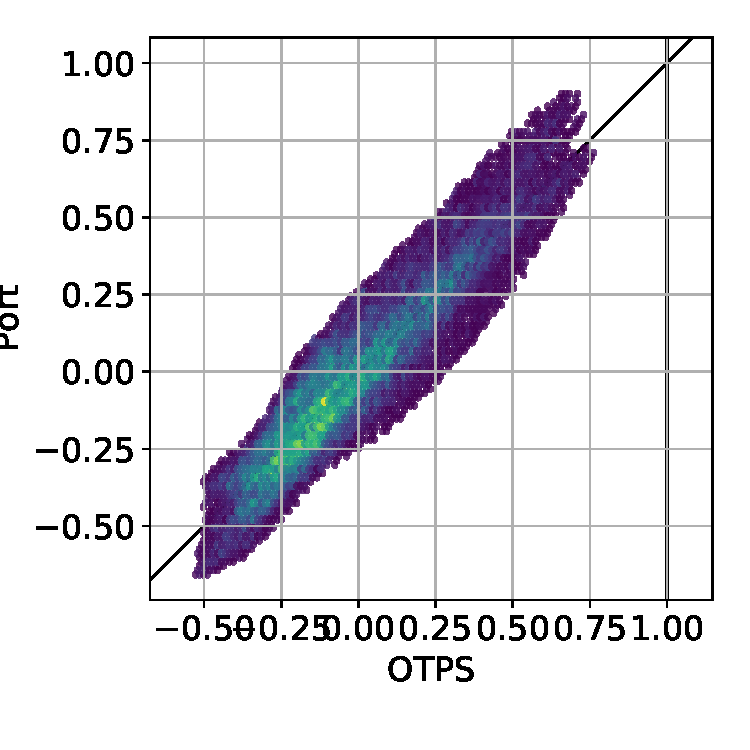
\includegraphics[height=0.25\textheight]{figures/plots/compareTides_61561_Full2020.pdf}
        \\
        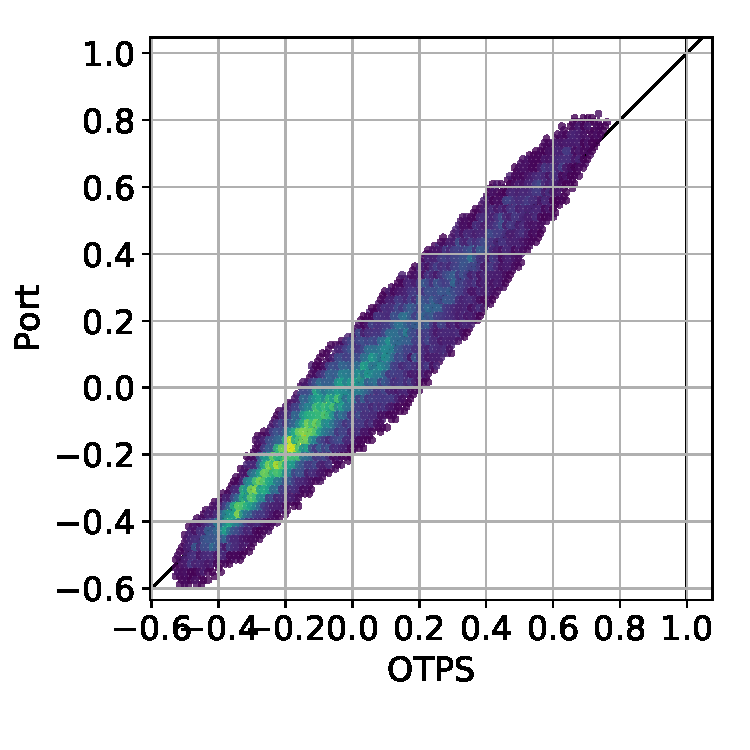
\includegraphics[height=0.25\textheight]{figures/plots/compareTides_61561_2020_201.pdf}
        \\
        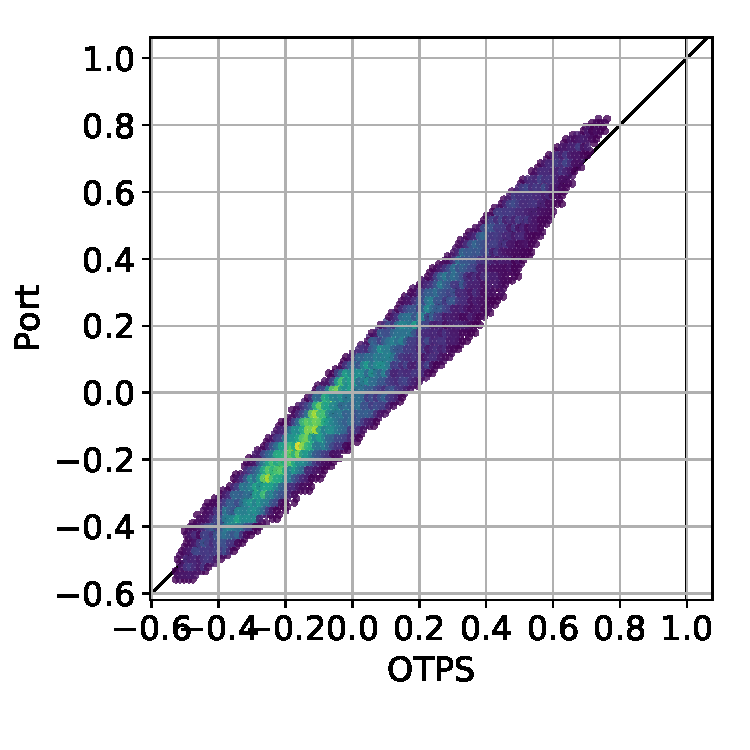
\includegraphics[height=0.25\textheight]{figures/plots/compareTides_61561_2020_105.pdf}
      \end{figure}
    \end{column}
\end{columns}
\end{frame}
%-----------------------------------------
\begin{frame}
\frametitle{Tidal service split}
      \begin{figure}      
        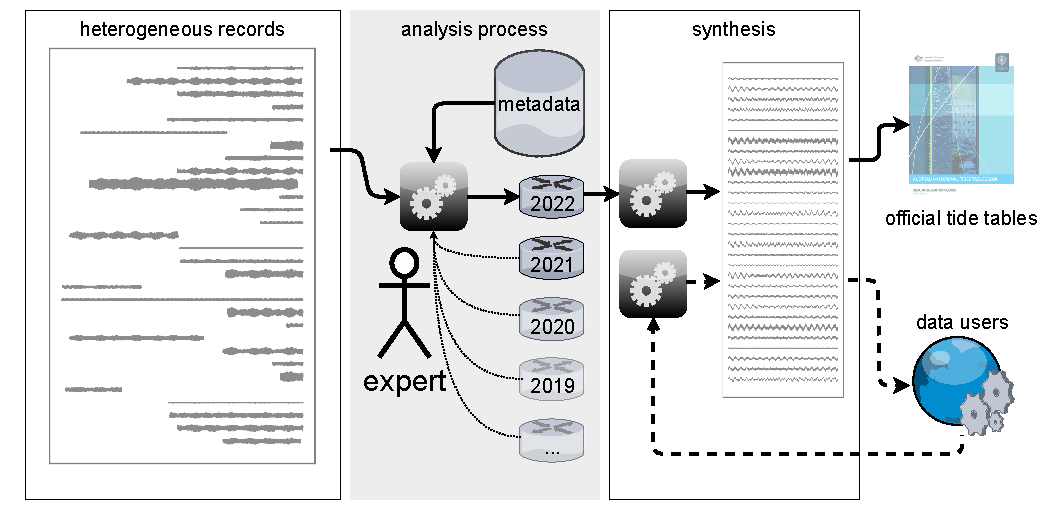
\includegraphics[height=0.6\textheight]{figures/diagrams/tideSchematic.pdf}
      \end{figure}
\end{frame}
%--------
\section{Wrap-up}
\begin{frame}
\frametitle{Wrap-up}
Mesoscale ocean has ``tidal'' relevance
\begin{multicols}{2}
\tiny

\begin{itemize}
    \item Incompatible definitions of ocean ``tide'' are in parallel operational use;
    \item despite spatial scale limitations, mesoscale ocean forecasts can directly provide significant forecast value for coastal sea level, but with many caveats;
    \item nominally tidal signals are present in mesoscale non-tidal ocean simulations and require care to avoid misinterpretation; 
    \item a simple aggregation approach to existing heterogeneous data provides an important skill benchmark for future sea level forecast system development; 
    \item point-based bias correction characteristics indicates that coastally contiguous extensions to model aggregation are feasible;
    \item the coastal propagation characteristics of candidate forecast systems can be qualitatively evaluated and compared in a grid-independent waveguide projection; 
    \item a coastal waveguide projection offers a means to direct forecaster attention to signals of special relevance along the Australian mainland coast;
    \item conventional harmonic tide predictions are not redundant but require appropriate product differentiation to compliment modern applications and facilitate future refinement.
\end{itemize}
\end{multicols}
\normalsize
\end{frame}
%-----------------------------------------
\begin{frame}
\frametitle{Seamless services and simulations }
Predictability and scales.
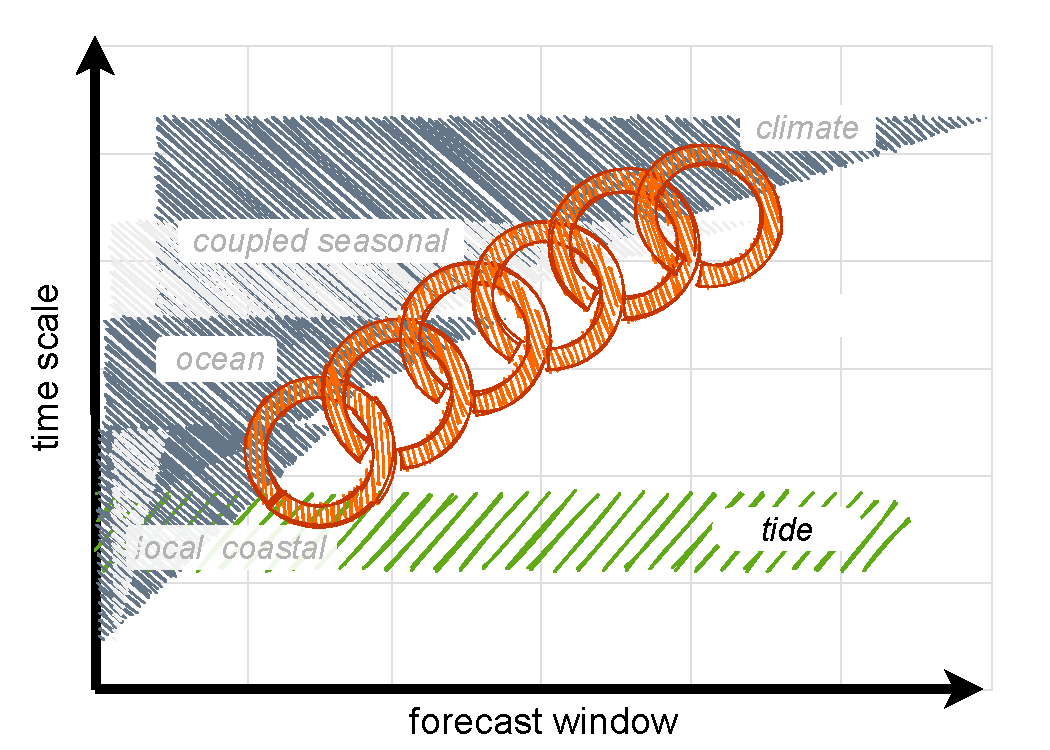
\includegraphics[height=0.7\textheight]{figures/diagrams/scales_with_chain_labelled.pdf}
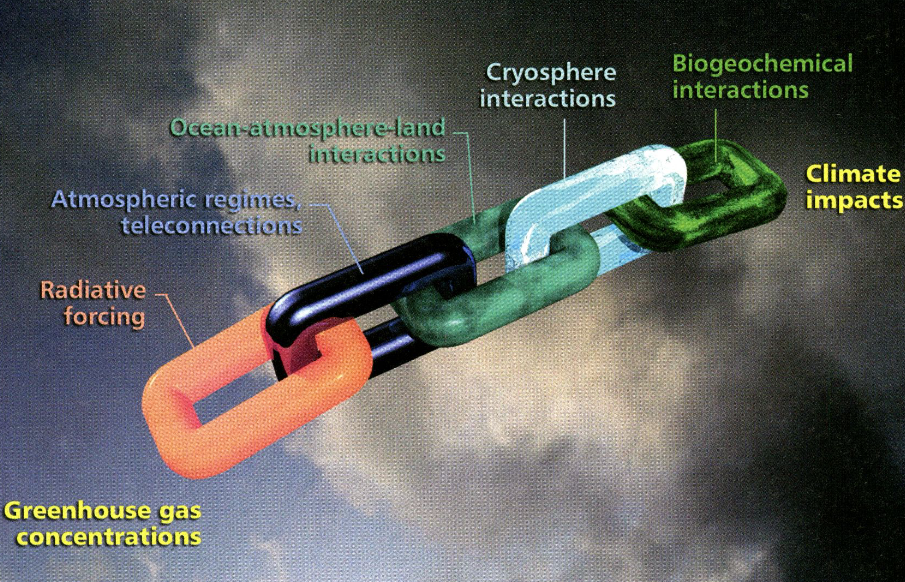
\includegraphics[height=0.2\textheight]{figures/images/PalmerChain.png}
\end{frame}
%-----------------------------------------
\begin{frame}
\frametitle{Thesis focus on one overlap}
     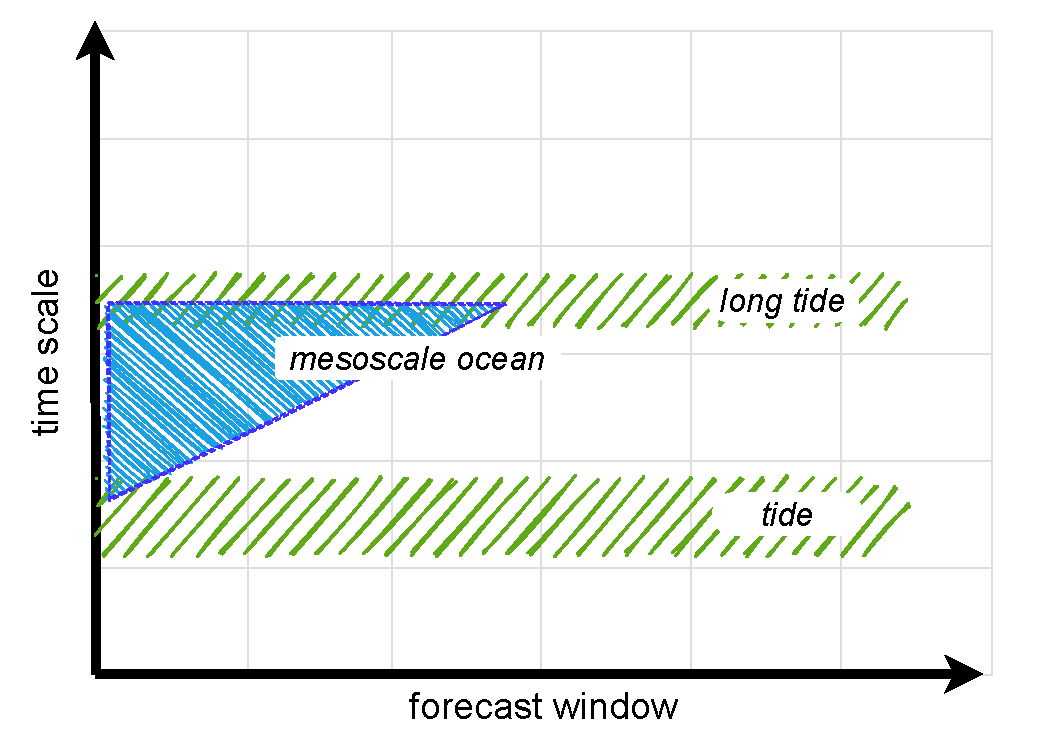
\includegraphics[height=0.7\textheight]{figures/diagrams/scales_focus.pdf}
\end{frame}
%-----------------------------------------
\begin{frame}
\frametitle{Thesis focus highlights: practical seamless not tidy}
\begin{minipage}{1.0\textwidth}
    \begin{itemize}
        \item downscaling chain good approach ...with limitations
        \item compatibility of signal representation particular 
        \item should plan for hybrids
    \end{itemize}
\end{minipage}
\hfill
\begin{minipage}{1.0\textwidth}
\begin{columns}
    \begin{column}{0.4\textwidth}
    \begin{figure}      
        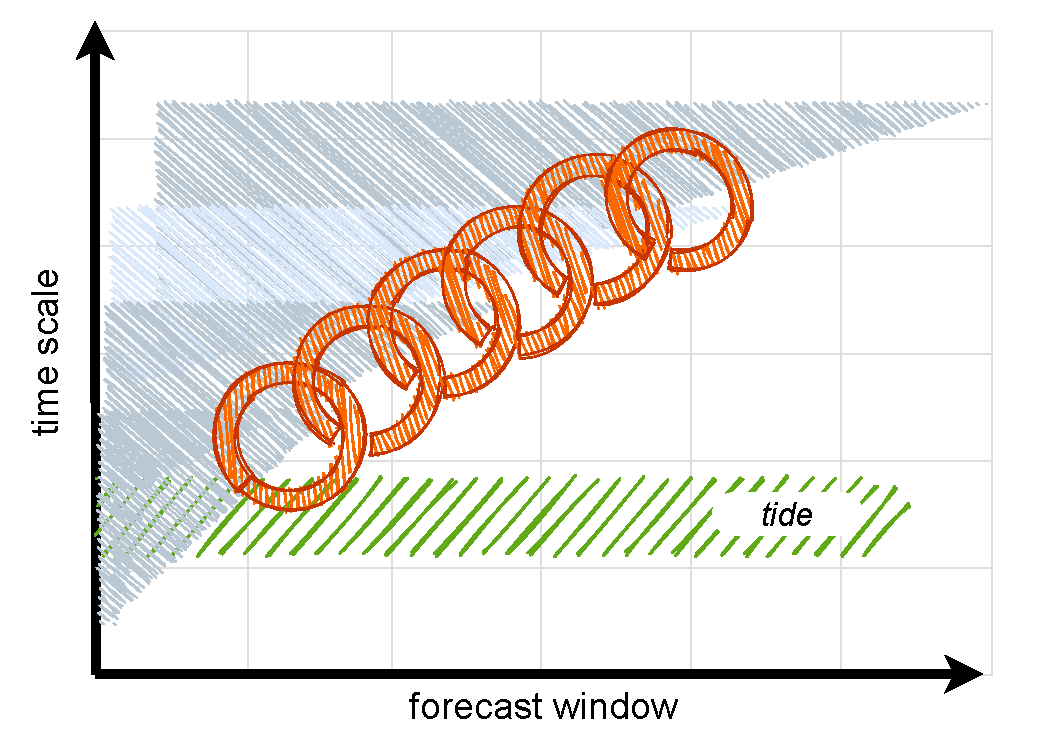
\includegraphics[width=\textwidth]{figures/diagrams/scales_with_chain.pdf}
    \end{figure}
    \end{column}

    \begin{column}{0.4\textwidth}
    \begin{figure}      
        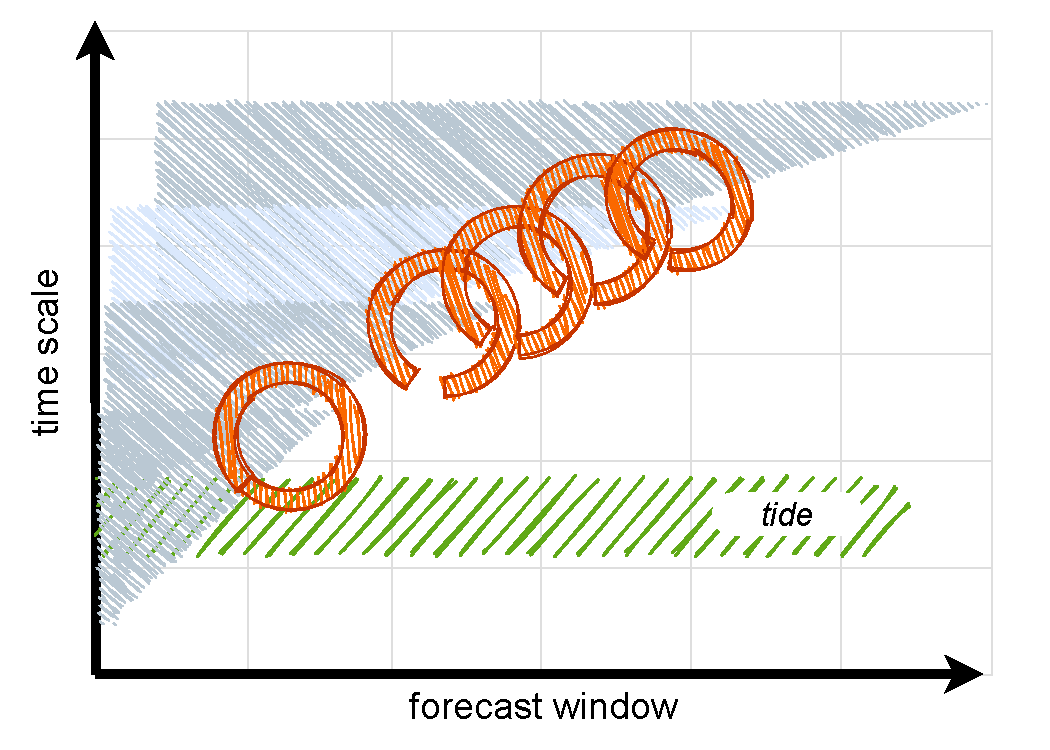
\includegraphics[width=\textwidth]{figures/diagrams/scales_with_broken_chain.pdf}
    \end{figure}
    \end{column}
    
\end{columns}
\end{minipage}

\end{frame}
\begin{frame}
\frametitle{Questions}
Thanks

\end{frame}
%------------------------------------------------------------
\end{document}



